\documentclass[12pt,oneside]{book}

\usepackage{mathtools,amssymb,amsthm,amsmath}
\usepackage{fancyhdr,setspace}
\usepackage{titlesec,graphicx}
\usepackage[margin=1in]{geometry}

\onehalfspace
\setlength{\parskip}{12pt plus 1pt minus 2pt}

\titleformat{\chapter}[hang]{\normalfont\bfseries}{}{0pt}{\huge}
\titleformat{\section}[hang]{\Large\bfseries}{\thesection\quad}{0pt}{\Large}
\newcommand{\iit}[1]{\textit{#1}}
\newcommand{\pit}[1]{(\textit{#1})}

\begin{document}

\frontmatter

\noindent Project Gutenberg's Four Lectures on Mathematics, by Jacques Hadamard \par

\noindent This eBook is for the use of anyone anywhere at no cost and with almost no restrictions whatsoever.
You may copy it, give it away or re-use it under the terms of the Project Gutenberg License included
with this eBook or online at www.gutenberg.org \par

\pagebreak

\noindent Produced by Andrew D. Huang, Brenda Lewis and the Online Distributed Proofreading Team at http://www.pgdp.net
(This file was produced from images from the Cornell University Library: Historical Mathematics Monographs collection.) \par
\vfill
\begin{center}
    Transcriber's Notes
\end{center}
\noindent In Lecture IV, equation (2) on p. 47, and equation (3) with its surrounding text on p. 52, are reproduced
faithfully from the original. \par

\noindent Except as noted above, minor typographical corrections and regularizations of spelling and mathematical
notation have been made without comment. This eBook may be easily recompiled with errors and irregularities
retained. Please consult the preamble of the \LaTeX\ source file for instructions. \par

\noindent Figures may have been moved slightly with respect to the surrounding text. \par

\noindent This PDF is formatted for printing, but may be easily formatted for screen viewing. Again,
please see the preamble of the source file for instructions. \par

\begin{titlepage}
    \centering
    {\large COLUMBIA UNIVERSITY IN THE CITY OF NEW YORK \par}
    {\normalsize PUBLICATION NUMBER FIVE OF\\THE ERNEST KEMPTON ADAMS FUND\\FOR PHYSICAL RESEARCH\par}
    {\normalsize ESTABLISHED DECEMBER 17TH, 1904 \par}
    \vspace*{-\baselineskip}
    \noindent\makebox[\linewidth]{\rule{14cm}{0.4pt}}
    {\Huge \textbf{FOUR LECTURES\\ON MATHEMATICS} \par}
    \vspace{1cm}
    {\large DELIVERED AT COLUMBIA UNIVERSITY\\IN 1911 \par}
    \vspace{2cm}
    {\normalsize BY \par}
    \vspace*{-\baselineskip}
    {\large J. HADAMARD \par}
    \vspace{0.5cm}
    {\tiny MEMBER OF THE INSTITUTE, PROFESSOR IN THE COLL\'EGE DE FRANCE AND IN THE \'ECOLE POLYTECHNIQUE,\\
    LECTURER IN MATHEMATICS AND MATHEMATICAL PHYSICS IN COLUMBIA UNIVERSITY FOR 1911}
    \vfill
    {\large NEW YORK\\COLUMBIA UNIVERSITY PRESS\\1915}
\end{titlepage}

\begin{center}
    Copyright 1915 by Columbia University Press
\end{center}

\pagebreak

On the seventeenth day of December, nineteen hundred and four, Edward Dean Adams, of New York, established
in Columbia University ``The Ernest Kimpton Adams Fund for Physical Research'' as a memorial to his son,
Ernest Kempton Adams, who received the degrees of Electrical Engineering in 1897 and Master of Arts in 1898,
and who devoted his life to scientific research. The income of this fund is, by the terms of the deed of gift,
to be devoted to the maintenance of a research fellowship and to the publication and distribution of the
results of scientific research on the part of the fellow. A generous interpretation of the terms of the deed
on the part of Mr. Adams and of the Trustees of the University has made it possible to issue these lectures as
a publication of the Ernest Kempton Adams Fund. \par
\noindent\makebox{\rule{16.5cm}{1pt}}

\pagebreak
\chapter{Preface}
\noindent The ``Saturday Morning Lectures'' delievered by Professor Hadamard at Columbia University
in the fall of 1911, on subjects that extend into both mathematics and physics, were taken down
by Dr. A. N. Goldsmith of the College of the City of New York, and after revision by the author in 1914
are now published for the benefit of a wider audience. The author has requested that his thanks be expressed
in this place to Dr. Goldsmith for writing out and revising the lectures, and to Professor Kasner of Columbia
for reading the proofs. \par

\tableofcontents

\mainmatter

\chapter[Lecture I]{Lecture I\\
The Determination of Solutions of Linear Partial Differential Equations by Boundary Conditions}
\vspace*{-\baselineskip}
In this lecture we shall limit ourselves to the onsideration of linear partial differential equations
of the second order. \par

It is natural that general solutions of these equations were first sought, but such solutions have
proven to be capable of successful employment only in the case of ordinary differential equations.
In the case of partial differential equations employed in connecction with physical problems,
their use must be given up in most circumstances, for two reasons: first, it is in general impossible
to get the general solution or general integral; and second, it is in general of no use even when it
is obtained. \par

Our problem is to get a function which satisfies not only the differential equation but also other
conditions as well; and for this the knowledge of the general integral may be and is very often
quite insufficient. For instance, in spite of the fact that we have the general solution of Laplace's
equation, this does not enable us to solve, without further and rather complicated calculations,
ordinary problems depending on that equation such as that of electric distribution. \par

Each partial differential equation gives rise, therefore, not to one general problem,
consisting in the investigation of all solutions altogether, but to a number of definite problems,
each of them consisting in the reserach of one peculiar solution, defined, not by the differential equation alone,
but by the system of that equation and some accessory data. \par

The question before us now is how these data may be chosen in order that the problem shall be ``correctly set.''
But what do we mean by ``correctly set''? Here we have to proceed by analogy. \par

In ordinary algebra, this term would be applied to problems in which the number of the conditions is equal to that
of the unknowns. To those our present problems must be analogous. \textit{In general}, correctly set problems in
ordinary algebra are characterized by the fact of having soultions, and in a finite number. (We can even characterize
them as having a unique solution if the problem is linear, which case corresponds to that of our present study.)
Nevertheless, a difficulty arise on account of exceptional cases. \par

Let us consider a system of linear algebraic equations:
\begin{equation}
    \label{LinAl}
    a_1x_1 + \dots\ldots + a_nx_n = b_1\ldots \\
\end{equation}
the number \textit{n} of these equations being precisely equal to the number of unknowns.
If the determinant formed by the coefficients of these equations is not zero, the problem has only one solution.
If the determinant is zero, the problem is in general impossible. At a first glance, this makes our aforesaid
criterion ineffective, for there seems to be no difference between that case and that which the number of equations
is greater than that of the unknowns, where impossibility also generally exists. (Geometrically speaking, two straight
lines in a plane do not meet if they are parallel, and in that they resemble two straight lines given arbitrarily
in three-dimensional space.) The difference between the two cases appears if we chose the \textit{b}'s (second
members of the equation \ref{LinAl}) properly; that is, in such manner that the system becomes again possible.
If the number of equations were greater than \textit{n}, the solution would (in general) again be unique; but,
if those two numbers are equal, the problem when ceasing to be impossible, proves to be \textit{indeterminate}. \par

Things occur in the same way for every problem in algebra. For instance, the three equations
\begin{align*}
    f(x,y,z)&=a \\
    g(x,y,z)&=b \\
    f+g&=c
\end{align*}
between the three unknowns $x$, $y$, $z$, constitute an impossible system if $c$ is not equal to $a+b$, but if
$c$ equals $a+b$, that system is in general indeterminate. \par

Moreover, this fact has been both extended and made precise by a most beautiful theorem due to Schoenflies. \par

Let
\begin{equation}
    \label{eq1.2}
    f(x,y,z)=X, \ g(x,y,z)=Y, \ h(x,y,z)=Z
\end{equation}
be the equations of a space-transformation, the functions $f$, $g$, $h$ being continuous. Let us suppose that within a given sphere $(x^2+y^2+z^2=1,\text{ for instance})$, two points $(x,y,z)$ cannot give the same point $(X,Y,Z)$: in other words, that $f(x,y,z)=f(x',y',z'),\ g(x,y,z)=g(x',y',z')=\ h(x,y,z)=h(x',y',z')$ cannot be verified simultaneously within that sphere unless $x=x',\ y=y',\ z=z'$. Let $S$ denote the surface corresponding to the surface $s$ of the sphere; that is, the surface described by the point $(X,Y,Z)$ when $(x,y,z)$ described $s$. If in equation (\ref{eq1.2}) we consider now $X,\ Y,\ Z$ as given and $x,\ y,\ z$ as unknown, our hypothesis obviously means that those equations cannot admit of more than one solution within $s$. Now \textit{Schoenflies' theorem} says that \textit{those equations will admit of a solution} for any $(X,Y,Z)$ that may be chosen within $S$. Of course the theorem holds for spaces of any number of dimensions. It is obvious that this theorem illustrates most clearly the aforessaid relation between the fact of the solution being \textit{unique} and the fact that that solution necessarily exists.\footnote{We must note nevertheless, that in it the unique solution is opposed not only to solutions in infinite number (as above), but also to any more than one. For instance, the fact that $x^2=X$ may have no solution in $x$, is, from the point of view of Schoenflies' theorem, in relation with the fact that for other values of $X$, it may have two solutions.} \par

As said above, the theorem is in the first place remarkable for its great generality, as it implies concerning the functions $f,\ g,\ h$ no other hypothesis but that of continuity. But its significance is in reality much more extensive and covers also the functional field. I consider that its generalizations to that field cannot fail to appear in great number as a consequence of future discoveries. This remarkable importance will be my excuse for digressing, although the theorem in question is only indirectly related to our main subject. The general fact which it emphasizes and which we stated in the beginning, finds several applications in the questions reviewed in this lecture. It may be taken as a criterion whether a given linear problem is to be considered as analogous to the algebraic problems in which the number of equations is equal to the number of unknown. This well be the case always when the problem is possible and determinate and sometimes even when it is impossible, if it cannot cease (by further particularization of the data) to be impossible otherwise than by becoming indeterminate.\label{pg4} \par

Let us return to partial differential equations. Cauchy was the first to determine one solytion of a differential equation from initial conditions. For an ordinary equation such as $f(x,y,dy/dx,d^2y/dx^2)=0$, we are given the values of $y$ and $dy/dx$ for a particular value of $x$. Cauchy extended that result to partial differential equations. \par

Let $F(u,x,y,z,\partial u/\partial x, \partial u/\partial y, \partial u/\partial z,\partial^2u/\partial x^2,\dots)=0$ be a given equation of the second order and let it be granted that we can solve it with respect to $\partial^2u/\partial x^2$. Thus we obtain $(\partial^2u/\partial x^2) + F_1 =0$ where $F_1$ is a function of all the above quantities, except $\partial^2u/\partial x^2$. Then Cauchy's problem arises by giving the values
\begin{equation}
    \label{eq3}
    u=\varphi (y,z),\ \frac{\partial u}{\partial x}=\psi(y,z)
\end{equation}
of $u$ and $\partial u/\partial x$ for $x=0$. (These data must be replaced by analogous data, if instead of the plane $x=0$, we introduce another surface.) Indeed, under the above hypothesis concerning the possibility of solving the equation with respect to $\partial^2 u/\partial x^2$, and on the supposition that the functions $F_1$, $\phi \text{ and } \psi$ are holomorphic, Cauchy, and after him, Sophie Kowalevske, showed that in this case there is indeed one and only one solution. This solution can be expanded by Taylor's series in the form $u=u_0+xu_1+x^2u_2+ \dots$ where $u_0,\ u_1, \dots$ can be calculated. \par

The above theorems are true for must equations arising in connection with physical problems, for example
\begin{equation}
    \tag{E}\label{E}
    \nabla^2u=\frac{\partial^2u}{\partial t^2}.
\end{equation} \par

\textit{But in general these theorems may be false}. This we shall realize if we consider Dirichlet's problem: to determine the solution of Laplace's equation
\begin{equation}
    \tag{e}\label{e}
    \nabla^2u=\frac{\partial^2u}{\partial x^2}+\frac{\partial^2u}{\partial y^2}+\frac{\partial^2u}{\partial z^2}=0
\end{equation}
for points within a given volume when given its values at every point of the boundary surface $S$ of that volume. \par

It is a known fact that this problem is a correctly set one: it has one, and only one, solution. Therefore, this cannot be the case with Cauchy's problem, in which \textit{both u} and one of its derivatives are given at every point of $S$. If the first of these data is by itself (in conjuenction with the differential equation) sufficient to determine the unknown function, we have no right to introduce any \textit{other} supplementary condition. How is it therefore that, by the demonstration of Sophie Kowalevska, the same problem with both data proves to be possible? \par

Two discrepancies appear between the sense of the question in one case and in the other: (\textit{a}) In the theorem of Sophie Kowalevska, $u$ has only to exist in the immediate neighborhood of the initial surface $S$. In Dirichlet's problem, it has to exist and to be well determined in the whole volume limited by $S$. We therefor require more in the latter case than in the former, and it might be thought that this is sufficient to resolve the apparent contradiction met with above. \par

In fact, however, this is not the case and we must also take account of the second discrepancy. (\textit{b}) The data, in the case of the Cauchy-Kowalevske demonstration, are, as we said, supposed to be analytic: the functions $\varphi,\ \psi$ (second members of (\ref{eq3})) considered as functions of $y,\ z$, are taken as given by convergent Taylor's expansions in the neighborhood of every point of the plane $x=0$ in the region where the question is to be solved. Nothing of the kind is supposed in the study of Dirichlet's problem. Not even the existence of the first derivatives of $u$, corresponding to displacements on $S$, is postulated, and in some researches, certain discontinuities of these values are admitted. Both these circumstances play their role in the explanation of the difference between the two results discussed above. \par

That (\textit{a}) is one reason for that difference is evident, for of course, if a function is required to be harmonic (i.e. to admit everywhere derivatives and to verify Laplace's equation) within a sphere, its values and those of its normal derivative, may not together be chosen arbitrarily on the surface even if analytic. \par

To show that \pit{a} is not sufficient for the required explanation, let us take the geometric terms of the problem in the same way as Cauchy. We therefore suppose that, \iit{u} being defined by Laplace's equation, the accessory data given to determine it are the values of \iit{u} and $\partial u/\partial x$ on the plane $x=0$, or, more exactly, on a certain portion $\Omega$ of that plane; $u$ will also not be required, now, to exist in the whole space; its domain of existence may be limited, for instance, to a certain distance, however small, from our plane $x=0$ (in the environs of $\Omega$) provided that distance be finite and not infinitesimal. \par

Now under these conditions, in general such a function $u$ does \iit{not} exist, if the data are not analytic and are chosen arbitrarily. One sees then a fact which never appeared as long as ordinary differential equations were alone concerned, namely, that the results are utterly different according as the analytic character of the data is postulated or not. \par

Of these two opposite results which is to be considered as giving us a more correct and adequate idea of the nature of things? I do not say as the true one, for of course each one is so under proper specifications. \par

Som mathematicians still incline to prefer the old point of view of Cauchy, one of their reasons being that, as known since Weierstrass, any function, analytic or not, can be replaced with any given approximation by an analytic one, (more precisely by a polynomial). Therefore the fact that a function belongs to one or the other of those two categories seems to them to be immaterial. I cannot agree with this point of view. That the thing is \iit{not} immaterial, seems to me to follow directly from what we have just stated. And it cannot fail to be put in evidence if we think not only of the mere existence of the solution, but of its properties and the means of calculating it. If Cauchy's problem, for equation (\ref{e}), ceases to be possible, as a rule, when the functions disgnated by $\varphi,\psi$ are not analytic, then every expression for the solution must depend essentially on that analyticity and especially upon the radii of convergence of the developments of $\varphi,\psi$. In other words, let us imagine that the functions $\varphi,\psi$ be replaced by other functions $\varphi_1,\psi_1$, the differencces $\varphi_1-\varphi,\psi_1-\psi$ being very small for every system of real values of $y,x$ within $\Omega$ (and perhaps also the differences of some derivatives being small). However slight the alteration may be it rigorously follows from the aforesaid theorem of Weierstrass, that the radii of convergence of the developments in power series (if existing at all) may and will be, in general, completely changed; so the calculations leading to the solution will necessarily be changed also. \par

If that solution itself should undergo but a slight change, this would at once show us that these methods of calculation ought to be of quite an artificial nature, masking completely the qualitative properties of the required result.\footnote{The solution by development in Taylor's series is, in general, for problems of that kind, the only one which can be given. I know but one exception, which is Schwarz's method for minimal surfaces, when a curve on the surface and the corresponding succession of tangent planes are given. This method rests on the favorable and exceptional circumstance that complex variables can be employed for the study of real points of such a surface.} But in fact, it is clear that matters are not as just assumed above. The alteration $u_1-u$ produced on the values of $u$ by our slight modification of $\varphi,\psi$ will be genneraly important and often complete, as is evident\footnote{If $u_1-u$ should be uniformly very small at the same time as $\varphi_1-\varphi,\psi_1-\psi$, it follows from the well-known convergence theorem of Cauchy that, letting the analytic functions $\varphi_1,\psi_1$, converge towards certain (non-analytic) limiting functions $\varphi,\psi$, the corresponding solution $u_1$ ought to converge uniformly towards a certain limit $u$, which would be a solution of the problem with the data $\varphi,\psi$.} by the fact that $u$ will cease completely to exist when $\varphi,\psi$ become non-analytical. This proves, first of all, that the application of Weierstrass' theorem in that case is illegitimate, since it gives an approximation for the data but nothing of the kind for the unknkown. \par

Then we see also that such a problem and calculation, the results of which are utterly changed by an infinitesimal error in starting, can have no meaning in their applications. \par

This leads to my second and chief reason for considering only the results which correspond to non-analytic data, namely, the remarkable accoerdance between them and the results to which physical applications bring us. \par

This accordance is the more interesting from the fact of its results being unexpected. Our former point of view--i.e. that of the Cauchy-Kowalevska theorem--evidently constitutes a complete analogy to the case of ordinary differential equations. But from our latter point of view--which is also the point of view in problems set by physical applications--every analogy seems to be upset. The results often seem almost incoherent; they will give opposite conclusions in apparently similar questions. \par

A first instance of this was given above. We know that Cauchy's problem is now impossible for Laplace's equation
\begin{equation}
    \tag{\ref{e}}
    \nabla^2u=\frac{\partial^2u}{\partial x^2}+\frac{\partial^2u}{\partial y^2}+\frac{\partial^2u}{\partial z^2}=0;
\end{equation}
but, on the contrary, in the equation of spherical waves
\begin{equation}
    \tag{\ref{E}}
    \nabla^2u=\frac{\partial^2u}{\partial t^2},
\end{equation}
or of the cylindrical waves
\begin{equation}
    \tag{E'}\label{E'}
    \frac{\partial^2u}{\partial x^2}+\frac{\partial^2u}{\partial y^2}-\frac{\partial^2u}{\partial z^2}=0,
\end{equation}
we may assign arbitrarily the values (whether analytical or not) of $u$ and $\delta u/\delta t$ for $t=0$, and Cauchy's problem set in that way has a solution (which is unique). In this latter case it is like a problem in algebra in which the number of equations is equal to the number of unknowns; in the former, like a problem in which the number of equations is superior\footnote{We could be tempted to apply in that case the remark made in the beginning (\ref{pg4}) concerning such impossible problems, which, notwithstanding that circumstance, must be considered as resembling ``correctly set'' ones. This, however, is not really applicable; for we have seen that the category alluded to is recognized by the fact that the problem may, under more special circumstances, become indeterminate. Now, this can never be the case in the present question: it follows from a theorem of Holmgren (``Archiv f\"ur Mathematik'') that the solution of Cauchy's problem, if existent, is in every possible case unique.} to the number of unknowns. \par

It never could have been imagined a \iit{priori} that such a difference could depend on the mere changing of sign of a coefficient in the equation. But it is entirely conformable to the physical meaning of the equations. Equation (\ref{E'}), for instance, governs the small motions of a homogeneous and isotropic medium, like a homogeneous gas; and the corresponding Cauchy's problem, enunciated above, represents the definition of the motion by giving the state of positions and speeds at the origin of times. On the contrary, equation (\ref{e}), which also governs many physical phenomena, never leads to problems of that kind but exclusively to problems of the Dirichlet type. The analytical criterion by which those two kinds of partial differential equations are to be distinguished, is known: it is given by what are called the \iit{characteristics of an equation}. The characteristics of an equation correspond analytically with what the physicist calls the \iit{waves} compatible with this equation, and are calculated in the following way. Let a wave be represented by the equation $P(x,y,z,t)=0$. In the given equation, for instance if $\nabla^2u-1/a^2\cdot\partial^2u/\partial t^2=0$ and $\nabla^2u$ be replaced by ($\partial P/\partial x)^2+(\partial P/\partial y)^2+(\partial P/\partial z)^2$ and $-(1/a^2)(\partial^2u/\partial t^2)$ by $-(1/a^2)(\partial P/\partial t)^2$ the condition thus obtained is
\begin{equation*}
    \left(\frac{\partial P}{\partial x}\right)^2+\left(\frac{\partial P}{\partial y}\right)^2+\left(\frac{\partial P}{\partial z}\right)^2-\frac{1}{a^2}\left(\frac{\partial P}{\partial t}\right)^2=0
\end{equation*}
(which is a partial differential equation of the first order). It must be verified by the function $P$. When this holds, $P(x,y,z,t)=0$ is said to be a characteristic of the given equation. \par

For equation (\ref{E}), such characteristics exist (that is, are real); this case is called the \iit{hyperbolic one}. \par

Laplace's equation, $\nabla^2u=0$, on making the above substitution, leads to the equation
\begin{equation*}
    \left(\frac{\partial P}{\partial x}\right)^2 + \left(\frac{\partial P}{\partial y}\right)^2 + \left(\frac{\partial P}{\partial z}\right)^2 = 0
\end{equation*}
which has no real solution. Therefore, in this case there are no waves and we havet he so-called elliptic case.\footnote{An intermediate case exists $\nabla^2u-k(\partial u/\partial t)=0$. This is semi-definite and is termed the parabolic one (example: the equation of heat).} Cauchy's problem can be set for a hyperbolic equation, but not for an elliptic one. Does this mean that for a hyperbolic equation Cauchy's problem will always arise? No, the matter is not quite so simple. For instance, in equation (\ref{E}) or (\ref{E'}), we could not choose arbitrarily $u$ and $\partial u/\partial y$ for $x=0$; this would lead us again to an impossible problem (in the non-analytic case, of course). \par

The physical explanation of this lies in the fact that there are, besides the partial differential equation, two kinds of conditions determining the course of a phenomenon, viz., the initial and boundary conditions. The former are of the type of Cauchy and they alone intervene in Cauchy's problem quoted above for the equation of sound. \par

But the boundary conditions are always of the type of Dirichlet. They are the only ones which can occur in an elliptic equation, but even in a hyperbolic one they generally present themselves together with initial ones. This gives place to so-called \iit{mixed problems} where the two kinds of data (belonging respectively to the Cauchy and to the Dirichlet type) intervene simultaneously for the determination of the unknown. \par

In equation (\ref{E}), $t=0$ represents the origin of time and can give place to initial conditions, having the form of Cauchy. But no such conditions can correspond to $x=0$, which represents a geometri boundary. \par

More or less complicated cases can arise for various dispoisitions of the configurations, giving place to other paradoxical and apparently controductory results, which can however all be explained in the same way. Moreover, there are other types of linear partial differential equations,\footnote{The so-called \iit{non-normal} hyperbolic equations, such as
\begin{equation*}
    \frac{\partial^2u}{\partial x_1^2}+\dots \frac{\partial^2u}{\partial x_m^2} - \frac{\partial^2u}{\partial y_1^2}\dots \frac{\partial^2u}{\partial y_n^2}=0 \quad (m>1,n>1).
\end{equation*} }
which do not govern any physical phenomena. The determination of solutions has been studied\footnote{By Hamel (Inaugural Dissertation, G\"ottingen) and Coulon (thesis, Paris).} in the analytic case but no sort of determination of that kind for non-analytic data has been discovered hitherto. \par

We see that from this non-analytic point of view the accordance between mathematical results and the suggestions of physics holds perfectly. This accordance must not surprise us, for, as we saw above, it corresponds to the fact that a problem which is possible only with analytic data can have no physical meaning. But it reamins worth all out attention. No other example better illustrates Poincar\'e's views\footnote{Lectures delivered at the first Internation Mathematical Congress, Zurich, 1897; reproduced in ``La Valeur de la Sciences.''} on the help which physics brings to analysis as expressed by him in such statements as the following, ``It is physics which gives us many important problems, which we would not have though of without it,'' and ``It is by the aid of physics that we can foresee the solutions.'' \par

\chapter[Lecture II]{Lecture II\\Contemporary Reseaches in Differential Equations, Integral Equations, and Integro-Differential Equations}
\section{Partial Differential Equations and Integral Equations}
I reminded you at the end of the last lecture what indispensable help the physicist renders to the mathematician in furnishing him with problems. But that help is not always free from inconveniences, and the task of the mathematician is often a thankless one. Two cases generally occur: it may happen that the physical problem is easily soluble by a mere ``rule of three'' method, but if not, it is so extremely difficult that the mathematician despairs of solving it at all; and he will strive after that solution for two centuries and, when he obtains it, our interest in the particular physical problem may have been lost. Such seems to be the case with some problems concerning partial differential equations. Just after the discovery of infinitesimal calculus, physicists began by needing only very simple methods of integration, the problems in general reducing to elementary differential equations. But when high partial differential equations were introduced, the corresponding problems almost immmediately proved to be far above the level of those which contemporary mathematics could treat. \par

Indeed, those problems (such as Dirichlet's) exercised the sagacity of geometricians and were the object of a great deal of important and well-known work throught the whole of the nineteenth century. The very variety of ingenious methods applied showed that the question did not cease to preserve its rather mysterious character. Only in the last years of the century were we able to treat it with some clearness and understand its true nature. This clearness seemed to come too late, for at that time, physics began its present evolution in which it seems to disregard partial differential equations and to come back to ordinary differential equations, but of course in problems profoundly different from the simple cases which were familiar to Bernoulli or Euler. \par

Happily, for it would have been a humiliating thing to work so uselessly, this disregard was only in appearance, and the ancient problems have not lost their importance by the fact that other ones have been superposed on and not substituted for them. In fact, the solution now obtained for Dirichlet's problem has proved use ful in several recent researches of physics. \par

Let us therefore inquire by what device this new view of Dirichlet's problem and similar problems was obtained. Its perculiar and most remarkable feature consists in the fact that the partial differential equation is put aside and replaced by a new sort of equation, namely, the integral equation. This new method makes the matter as clear as it was formerly obscure. \par

In many circumstances in modern analysis, contrary to the usual point of view, the opeartion of integration proves a much simpler one than the operation of derivation. An example of this is given by integral equations where the unknown function is written under such signs of integration and not of differenetiation. The type of equation which is thus obtained is much easier to treat than the partial differential equation. \par

The type of integral equations corresponding to the plane Dirichlet problem is
\begin{equation}
    \label{2.1}
    \phi(x)-\lambda\int_A^B\phi(y)K(x,y)dy=f(x)
\end{equation}
where $\phi$ is the unknown function of $x$ in the interval$(A,B)$, $f$ and $K$ are knwon functions, and $\lambda$ is a known parameter. The equations of the elliptic type in many-dimensional space give similar integral equations, containing however multiple integrals and several independent variables. Before the introduction of eqwuations of the above type, each step in the study of elliptic partial differential equations seemed to bring with new difficulties; not only did the various methods imagined for Dirichlet's problem not cast more than a partial light on the equation, but the principles of most ofthem were peculiar to that special problem: they seemed to disappear if Laplace's equation was replaced by any other equation of the same type, or even (except for Neumann's method, which, as we shall soon see, is directly related to integral equations) if for the same Laplace's equation Dirichlet's problem was replaced by any analogous one such as presented by hydordynamics or theory of heat. Each of them, besides, was rather a proof of existence than a method of calculation. \par

Then they seemed again quite insufficient for another series of questions which mathematical physics had to solve, viz., the sutdy of harmonics. The existence of those harmonics (such as the different kinds of resonance of a room filled with air) was physically evident, but for the mathematician it offers an immense difficulty. Schwarz, Picard and Poincar\'e gave a first solution which was rather complicated as each harmonic requires for its definition a new infinite process of calculation after the preceding one has been determined. Nevertheless it has demonstrated rigorously the chief properties of the quantities in question (namely, certain special values of the parameter in equation (\ref{2.1})), i.e. that they exist and form a discrete infinity, only a finite number of them lying within and finite interval. \par

But at the same time a discovery even more important, in a certain sense ,was made by Poincar\'e, namely the near relation between that question of harmonics and the method which had been indicated by Neumann for Dirichlet's problem. This discovery of Poincar\'e paved the way for Fredholm's work. The latter treats every one of the aforesaid questions, and any which can be assimilated to them, by one and the same method, which consists in the reduction to an equation such as (\ref{2.1}). This gives all the required results at once and for all the possible types of such problems. \par

In all this, the mathematician seems to play again the unfortunate r\^ole we alluded to in the beginning; for those results are nothing but the mathematical demonstration of facts each of ewhich was familiar to every physicist long before the beginning of all those researches. But of course their interest is not in fact limited in demonstration; they can and do serve as starting points for the discovery of new facts. They are useful as giving the proper method of calculation. Previously, in the calculation of the resonance of a room filled with air, the shape of the resonator had to be quite simple, which requirement is nota necessary one for the case where integral equations are employed. We need only make the elementary calculation of the function $K$ and apply to the function so calculated the general method of resolution of integral equations. \par

There are two chief methods for the solution of the equations. It is not always wasy to get numerical results. \par

Liouville and Neumann (in solving Dirichlet's problem) really worked out a method of solving integral equations. A second method is due to Fredholm. The first method leads to series which may converge slowly but they are easy to calculate. The method of Fredholm gives a quotient of two series (entire functions of $\lambda$) the terms of which have to be calculated independently, while in the first method each is obtained from the one immmediately, while in the first method each is obtained from the one immediately preceding it. While we must add that Erhard Schmidt has shown how the first method can be made to supply a more rapidly convergent series, Fredholm's method is of greater value to physics because of the theoretical point of view. It gives easily (what was impossible before its appearance) not only the existence of harmonics, but their properties. For instance, older methods could not have succeeded, at least not without great difficulties and a large amount of calculation, in obtaining the order of magnitude of the successive upper harmonics (i.e. the corresponding great values of $\lambda$). They would probably have been quite unable to predict the order o magnitude, as is done in the recent works of Hermann Wayl, so as to show its relation the volume of the room to which they correspond. But it has even proved of great importance for physics to know mathematically, and not only empirically, that the harmonics corresponding to equations of the form (\ref{2.1}) are a discrete infinity. For in the case of the spectral frequencies we get series which tend to accumulate towards definite positions. Since Fredholm's theory we can assert that such series are not compatible with the form of integral equation given at the beginning of this lecture. \par

Fredholm himself investigated new forms (as also did Walther Ritz). The introduction of the integral equation has made even the above problem accessible. The older method would not have been able to decide whether the distribution in question was possible or not. The hypothesis proposed by Fredholm leads to an integral equation such as
\begin{equation}
    \label{2.2}
    \phi(x)-\frac{1}{k-\lambda^2}\int_a^b\phi(y)K(x,y)dy=f(x)
\end{equation}
Here the frequencies will accumulate in the neighborhood of $\lambda=\sqrt{K}$. \par

I must immediately add that, as Ritz showed, Fredholm's type is not sufficient to give a correct explanation of the phenomena. But this does not change the essential fact that by the aid of the new method we are immediately able to decide what the asymptotic distribution of harmonics can or cannot be, so that comparison with observation becomes possible; and this we own entirely to Fredholm's method. \par

\section{Coming Back to Ordinary Differential Equations}
As we said in the beginning, the subject of partial differential equations which was the main and almost the only occupation of mathematical physics, ceases nowadays to be so. As a consequence of the general admission of the discrete structure of matter, physical problems tend now to lead to ordinary differential equations. These differential equations are to be studied under the most difficult circumstances because we must follow the form of the solutions for very long periods oftime, that is, of the independent variable $t$. One can say that such a study did not exist before Poincar\'e, and even his researches on the subject, I mean especially his four chief memoirs in the ``Journal de Mathemtiques,'' 1887 (\iit{On the shape of Curves Defined by Differential Equations}), lead us, like Socrates, to begin to feel that we know nothing. \par

We cannot, in this place, lay stress on the extraordinary complications and paradoxes which he discovered. We shall mention only one of them, because it helps to correct an error frequently committed in hydrodynamical and electrical problems, concerning the lines of force and the lines of flow. These lines are all defined by ordinary differnetial equations. The general form is $dx/X=dy/Y=dz/Z$. In a very general category of cases the vector $XYZ$ has the property that
\begin{equation*}
    \text{div}(XYZ)=\left(\frac{\partial X}{\partial x}+\frac{\partial Y}{\partial y}+\frac{\partial Z}{\partial z}\right)=0
\end{equation*}
Now, whenever such conditions existed, physicists used to say that the tubes of force--or tubes of flow, or tubes of vortices--were closed (if they did not go to infinity or come to the boundaries of the domain of existence of the vector $X,\ Y,\ Z$). \par

They were, I think led to say so by the examples given by some simple peculiar cases in which the differential equations could be integrated, for one could not suspect before Poincar\'e's work that such cases are exceptional, generally giving a quite inadequate and deformed view of things. In fact, the assertion in question is an utteryl false one.\footnote{A demonstration is frequently given to justify it, the error of which consists in an incomplete enumeration of possible cases.} If you allow me such a crude comparison, it is not true that the tube of force must get back home and put its key in the lock. Rather does it put its key above and below and on either side, and never succeeds in getting it in exactly. It will, it is true, nearly get back an infinite number of times. The only consequence which can be correctly drawn from the equation $\text{div}(XYZ)=0$ is that the area of the cross section of the tube cannot have changed. But its shape may, and generally will, have done so. If it were, let us say, circular in starting , it will have become elliptic when coming back and its ellipticity will increase at each return. Finally it will become a long flat strip and only a part of it will come back to the neighborhood of its original position. In Fig. 1, the successive appearances of the same tube of force are shown. The tube of force may have been originally circular, but on its first recurrence of return, it may have become elliptic in cross section and thus it has only partly returned to its original position. Still more is this that case in the second recurrence of the tube of force, which may be assumed by this time to have become very flat in cross section.

\begin{figure}
    \centering
    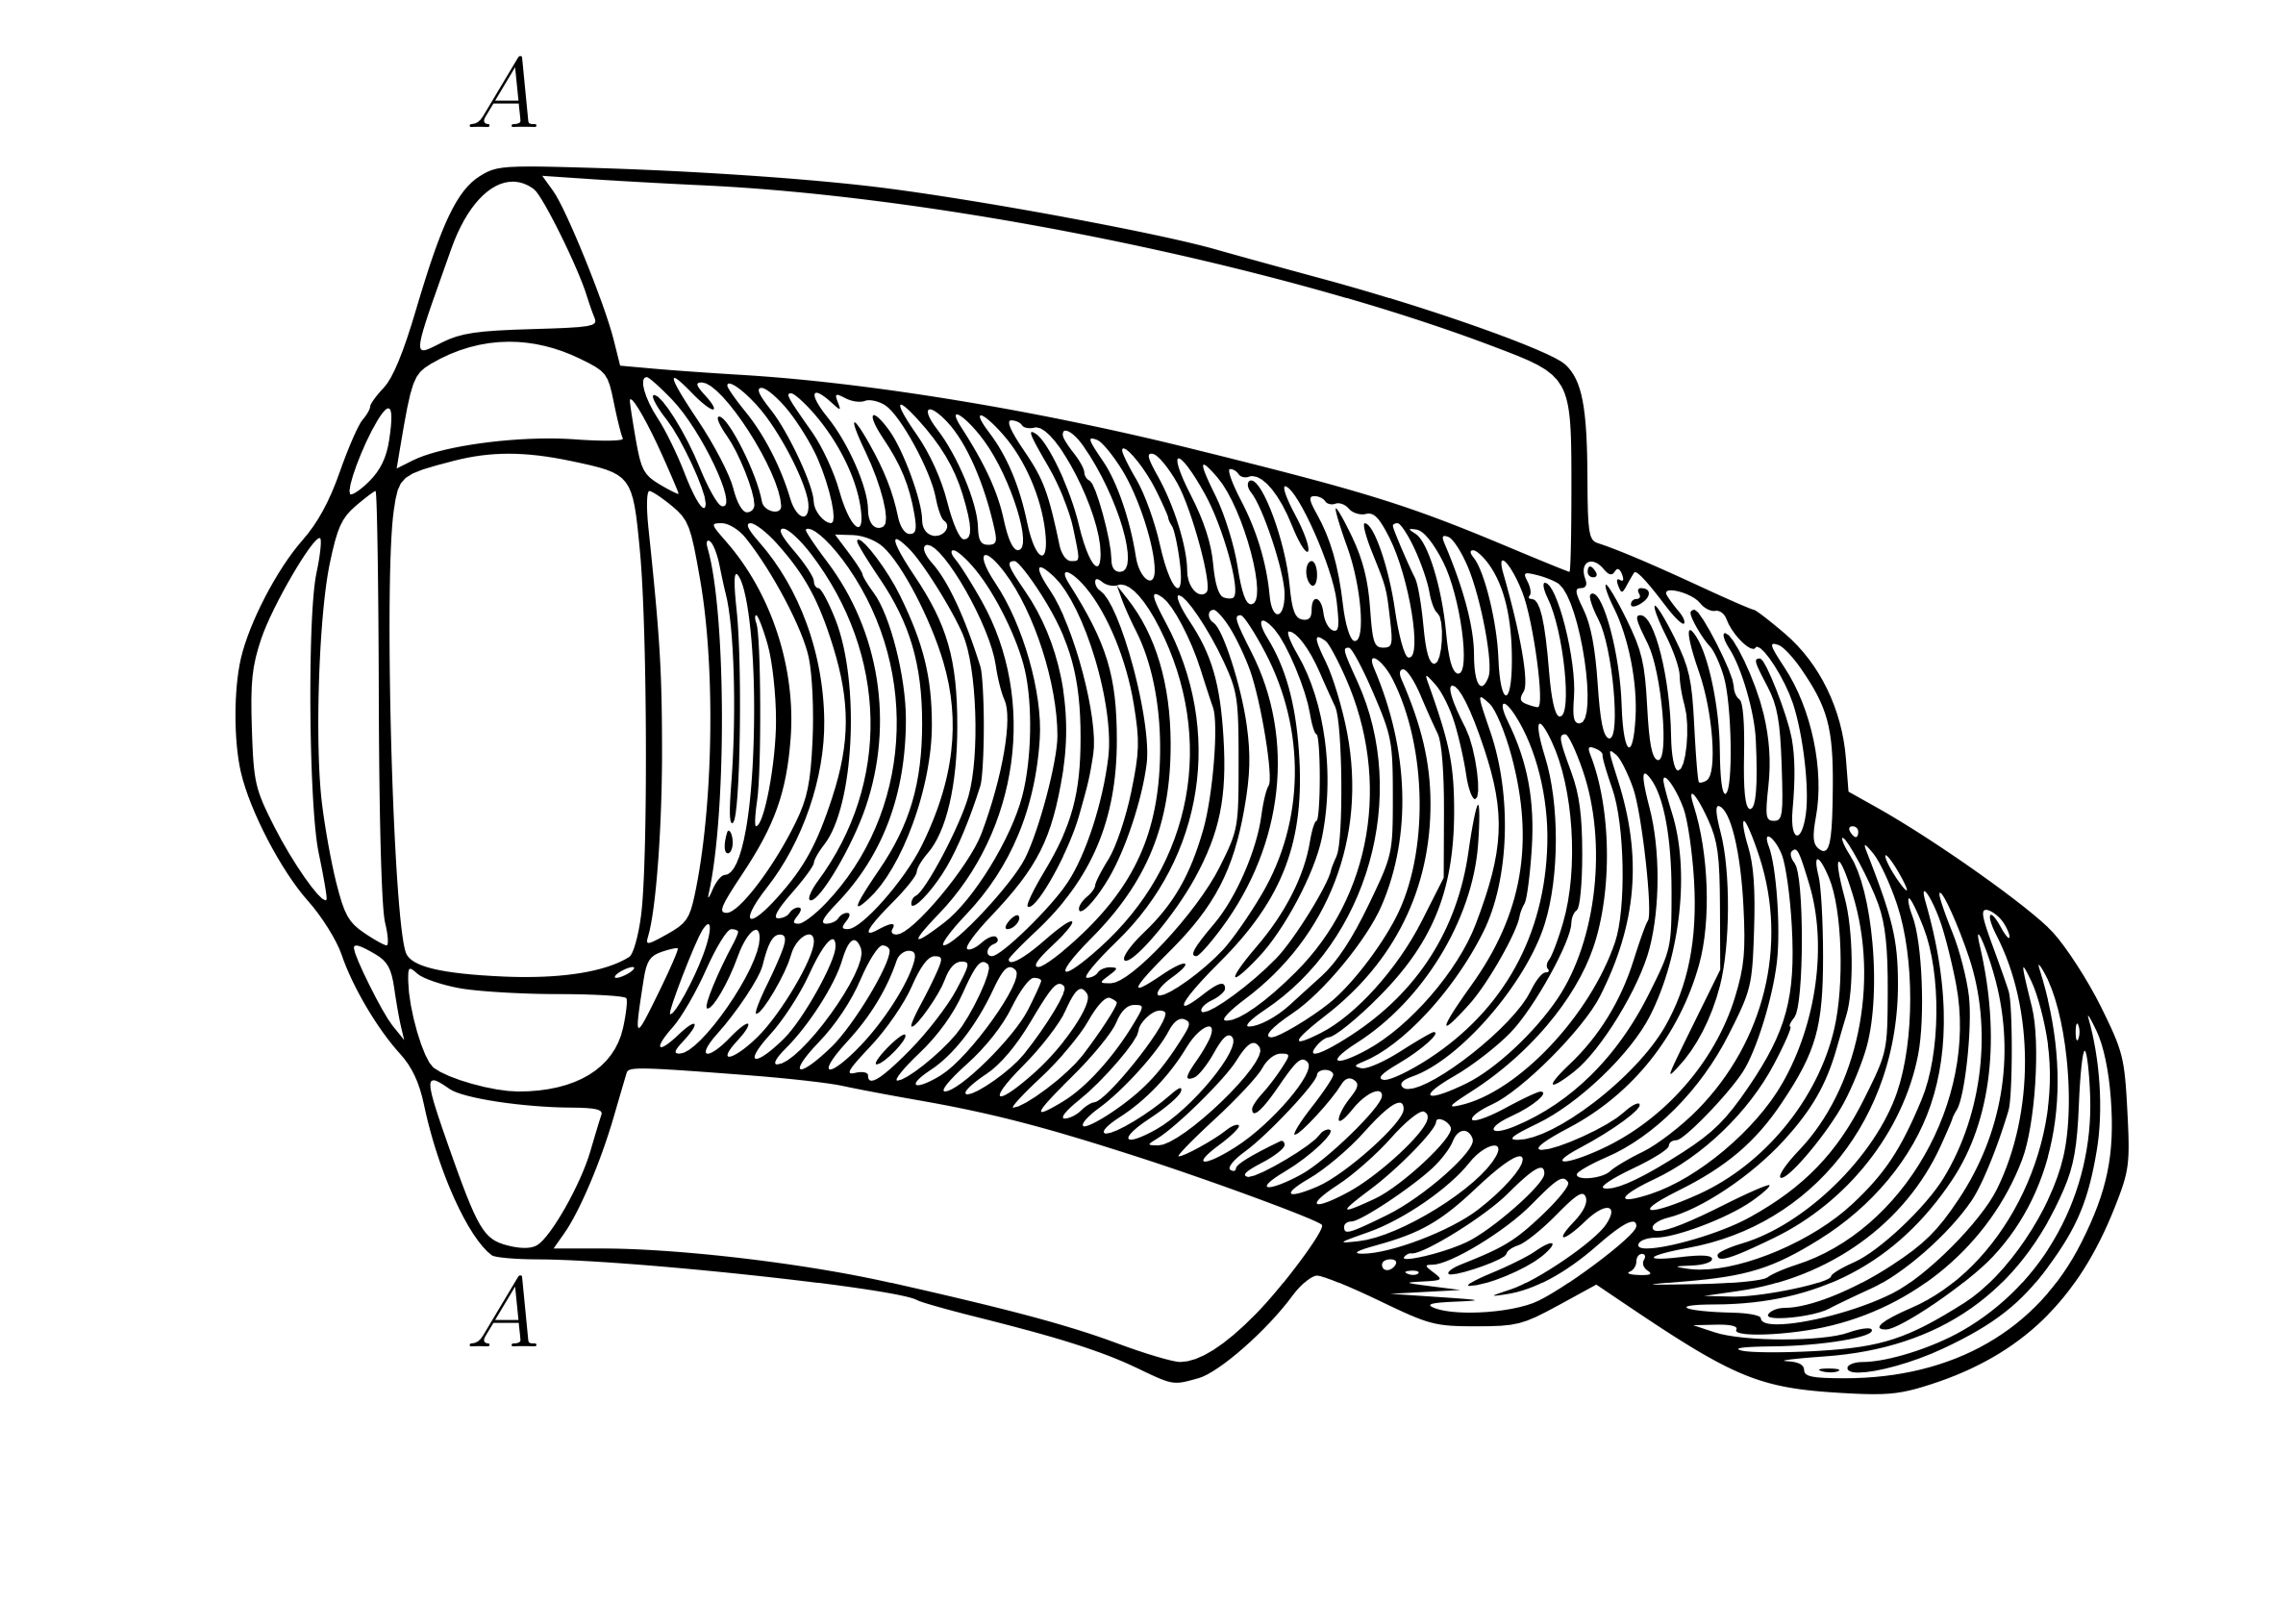
\includegraphics[height=10cm]{Fig1.jpeg}
    \caption{}
    \label{Fig1}
\end{figure}

As Mr. Birkhoff kindly pointed out to me, it is interesting to remark that in most cases, the deformed and falttened tube will even pass \iit{simultaneously} indefinitely near to any point of the considered medium. \par

A rather curious fact must nevertheless be stated. Although the principle that the tube is closed is completely false, the conclusions drawn from it by physicists are most often true. Why is this so? Perhaps the explanation lies in the fact that under the same hypothesis, div$(X,Y,Z)=0$, a line defined by our differential equations generally returns indefinitely near and an infinite number of times to its starting point. (This is called ``Stabilit\'e a la Poisson.'') Poincar\'e has shown that though not every line in question necessarily does this, the fact occurs for an infinitely greater number of cases than those in which it does not occur. \par

\section{Application to Molecular Physics}
We see by this single example how complicated and unexpected the shapes of curves defined by differential equations may be, and how far we are from understaning them when considered for great values of the independent variable. \par

But could we be satisfied with our work if we succeeded in doing so? This even is doubtful. I cannot help thinking of a bequest left to the French Academy of Science for a prize to the first person who should be able to communiate with a planet other than Mars! The case of molecular physics reminds me of that rather difficult requirement. The discussion of the molar effects (i.e. the effects on quantities of matter accessible to observation) of molecular movements is a mathematical problem, which, logically speaking, would presuppose a rather advanced knowledge of curves defined by differential equations, and take this as a starting point, in order to discuss the questions of probability connected with such curves. \par

That probabilty plays its role in the movements of almost any dynamical system, follows from the statements we just quoted. If the initial positions and the initial speeds of the moving points are exactly given, so will be the final positions and speeds after any (however long) given period of time. But if this period is long, and if we make a very small error in the initial conditions, the small error will have a muchmagnified effect and even cause a total change in the results at the end of the long period of time, and this is precisely Poincar\'e's conception of hazard. It is like a roulette game at Monte Carlo where we do not know all the conditions of launching the ball which induces the hazard. And so we know nothing more about the conditions than the gamblers. In other words, molecules are finally mixed just as cards after much shuffling. It is this fundamental hazard which plays the main part in Gibbs's method. A sort of mixing function ought to be introduced. Let us start on one of the lines of force. If we know exactly the point of departure $A$ we should know accurately the point of arrival. If $A$ is but approximately known, that point of arrival may occupy all sorts of positions; and indeed, in many differential problems, it may coincide (approximately) with any point $B$ within the domain where the differential system is considered (though this is exactly so for dynamical problems on account of the energy integral or other uniform integrals which the equations may admit.) \par

Therefore, the starting point being approximately $A$, there will be a certain probability that the point of arrival will be in a certain neighborhood of another given point $B$; and that probability will be a certain function of the positions of the two points $A,\ B$. \par

Now, logically speaking, in order to solve the question set for us by kinetic theories, we ought to take such a ``mixing function,'' assuming it to be known, as a base for further and perhaps complicated reasoning. In fact, the main present theories in statistical mechanics rest on certain assumptions concerning that function, which are very playsible. But, rigorously speaking, we are not able to consider them as theorems. \par

Happily, things are greatly simplified by the fact that in such mixings the aforesaid function, characteristic of the law of mixing, only intervenes by some of its properties and may be changed to a large extent without changing the final result. This is what Poincar\'e showed for the ordinary shuffling of cards in his ``Calcul des Probabilti\'es'' (second edition). In one shuffling the peculiar habits of the player certainly intervene and so do they more or less after only a few shufflings. But after many shufflings the results become totally independent of those habits. Poincar\'e also shows (though with some exceptions which do not however seem to play a great practical role), that such is likewise the case in the kind of mixing introdued by molecular theories. \par

Some known facts in the history of these theories give a striking instance of this. Such is the work of Blotzmann and Gibbs in the treatment of the kinetic theory of gases and statistical mechanics. They both obtained the result that if we consider the probability of the average number of molecults in 6-dimensional space and call it $P$, and integrate log$P$ over the whole mass, the conclusion drawn will be that the integral obtained is constantly increasing. Crtiics, and among them myu colleague and friend Brillouin, say: ``We have not to congratulate ourselves onf the result, because the two speak of quite different things and yet they agree. Gibbes does not mention the collision of molecules, while Boltzmann's analysis is founded on the collisions of molecules. The primitive order of the molecules is disturbed by such collisions and a mixing is produced. Gibbs gets a similar mixing by the mere consideration of differential equations existing over long periods of time.'' In both cases, if we consider systems which are ``molecularly organized,'' after a certain time the molecules will be so much less organized and more mixed up. \par

We are surprised to find this coincidence of the results of Gibbs and of Boltzmann in such circumstances. We shall, however, cease to consider it as fortuitous and perceive its true signification by precisely what we just remarked on the shuffling of cards, which makes us understand that such final results may and do depend on properties which are, in general, common to utterly various laws of mixing. \par

But the difficulties met with in partial or ordinary differential equations are not the only ones which we had to consider at the present time. The mathematicians have contrived to intoduce a new sort of equation, more difficult than the previous ones, the integro-differential equation. \par

\section{Integro-Differential Equations}
We are now forced to consider this new form. Here the unknown function simultaneously appears in integrals and in differentials. We have at least two completely different cases of such equations to consider. Their difference corrseponds to the two sorts of variables which intervene in all physical problems, the space variables $x,y,z$, and the time variable $t$. (There may be more than three variables in the first group.) \par

Type 1: Differentiation with respect to $x,y,z$; integration relative to $t$. Type 2: Differentiation with respect to $t$; integration relative to $x,y,z$. And even though this type dates only from 1907, we have already found cases of both kinds. \par

Volterra was led to consider the first one in connection with ``The Mechanics of Heredity.'' This is the case where the properties of the system depend on all the previous facts of its existence (such as magnetic hysteresis, straings of glass, and permanent deformations in general). \par

Volterra considers elastic hysteresis. Let $T$ by any component of strains; $E$ the component of deformation. (There are six $T$'s and six $E$'s.) Then formerly we considered $T_{hk}=\sum a_{hk}E+{hk}$. There are 6 equations of this type. There are 21, 36, 6 or 2 $a$'s depending on the theories. If we consider heredity, we must introduce new terms, Suppose that at the time 0 there were no strains; then $T_{hk}=\sum aE_{hk}+\int_0^t(\sum aE)_td\tau$ where $\tau$ is the variable time. This is an equation in which we have derivatives with respect to $x,y,z$, and an integral with respect to the time; and the same character subsists if, from those values of the $T$'s, we deduce the equations of movement. Water waves furnish us with an instance of the opposite type. One knows that waves on the surface of water are the most common examples of an undulatory phenomenon and that, for this reason, they are most frequently used to give to the beginner a first idea of what such phenomena are. \par

But it is a general, though astonishing fact, that the most simple of daily phenomena are the most difficult to understand. While the theory of a\"erial or even elastic waves is rather simple, at least as long as viscosity is left aside,\footnote{In a viscous gas, waves cannot exist, strictly speaking. They are replaced by quasi=waves which were first considered by Duhem, and more profoundly studied in an important memoir presented by Roy to the French Academy of Science.} and now classically reduced to analytical principles (related to notion of characteristics as we saw in the preceding lecture), the properties of surface waves in liquids are much more hidden. The few results classically known on that subject are even of a contrdictory nature. One of them is the differential equation given by Lagrange in the case of small (and constant) depth, which has served as a model for the dynamical theory of tides, the equation obtained as governing the phenomenon being in both cases a partial differential equation of the \iit{second} order. But, for the same phenomenon on a liquid of indefinite depth, Cauchy gets a partial equation of the \iit{fourth} order. The truth is that the problem does not lead to a differential equation at all, but to an integro-differential equation. For an orginally plane surface with small displacements, where $z$ is the vertical displacement at $(x,y)$, then
\begin{equation*}
    \frac{d^2z}{dt^2}=\iint Z_Q\phi(P,Q)dS_Q.
\end{equation*}
Thus, for any determinate point $P$ of the surface defined by its coordinates $(x,y)$ the vertical acceleration depends on the values of $z$ in every other point $Q(x',y')$. Here $S_Q$ is $dx'dy'$ and $\phi$ is a known function of $(x,y,x',y')$. The above equation is of the second form of integro-differential equations. \par

Volterra succeeded in the case of isotropic bodies in reducing the problem to the solution of a partial differential equation and an ordinary integral equation. But things are not so simple for crystalline media.\footnote{Since these lectures were delievered, Professor Volterra has given a comprehensive view of his methods and solutions in a course of lectures at the University of Paris. See the issue of those lectures by J. Peres (Paris, Gautheir Villars).} \par

The two types of integro-differential equations, which we just enumerated, are completely different in their treatment. Volterra's type resembles the partial differential equations (of the elliptic or sometimes parabolic genus in the examples hitherto given). The equation must be completed by accessory conditions which are nothing else than boundary conditions (cf. Lecture I). The methods given by Volterra run exactly parallel to those which are applied for Dirichlet's problem (such as the formation of Green's functions). \par

In the second type described above, the accessory considitions are initial ones; and are to be treated in the manner, not of partial, but of ordinary differential equations--such methods as Picard's successive approximations being of great use in that case. \par

\chapter[Lecture III]{Lecture III\\Analysis Situs in Connection with\\Correpondences and Differential Equations}
\section{}
We are going to speak of the role of analysis situs in our modern mathematics. This theory is also called the geometry of situation. It is the study of connections between different parts of geometrical configurations which are not altered by any continuous deformation. We suppose that we can let a system undergo any deformation whatever, however arbitrary it may be, only that it preserves continuity. For instace, a sphere and a cube are considered as one and the same thing from te point of view of the seometry of situation, because one can be transformed into the other without separating parts, or uniting parts which formerly were separated. The circle and the rectangle are identical from the same point of view. But the lateral surface of a cylinder and the surface of a rectangle are not identical, because, from the transformation of one into the other, we must make a cut along a generatrix. Also one is limited by two lines (the base circles) while the other is limited by one. The total surface of a cylinder is entirely closed; it is identical withe the surface of a sphere. There is no difficulty in the transformation. \par

If we consider the ``anchor ring,'' the case is different. This is a closed surface but it has a hole which is not found in the surface of the sphere, and the surface of the sphere cannot be transformed continuously in it. It would have to be transformed by several cuts, the first of them (\ref{Fig2}) giving a broken ring, which for us is identical with the lateral surface of a cylinder. This may be cut into a rectangle and then transformed into a sphere. But the transformation of an anchor ring into a sphere cannot be done without cutting and piecing. The principles of analysis situs, for surfaces in ordinary space, are well known and I do not intend to go over them at this moment. We shall take them for granted. According to them, a surface of two dimensions is defined from our present point of view by the number of boundaries and another number, namely the \textit{genus}. The genus is zero for the sphere and one for the anchor ring. For a pot with two ``ears'' (\ref{Fig3}) we have the genus two. \par

\begin{figure}
    \centering
    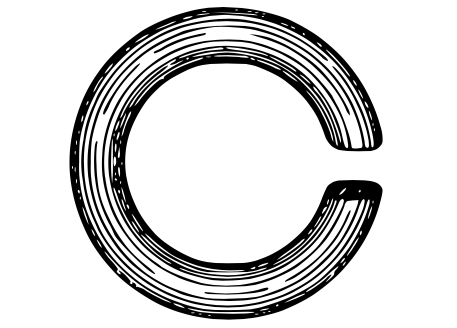
\includegraphics[height=10cm]{Fig2.png}
    \caption{}
    \label{Fig2}
\end{figure}

\begin{figure}
    \centering
    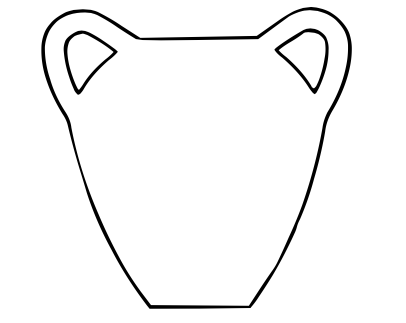
\includegraphics[height=8cm]{Fig3.png}
    \caption{A pot with two ears.}
    \label{Fig3}
\end{figure}

Analysis situs started with trifling problems, such as that treated by Euler of the bridges of K\"onigsberg over the Pregel river. There are seven bridges; the problem is to go over all of them without passing twice over any one (\ref{Fig4}). The great Euler did not disdain to occupy himself with this and many other apparently childish problems. But what interests us in this one especially is that it involves the geometry of the situation, in the sense in which we have used the term. For even if the islands in the rives had other shapes and the bridges had the queerest forms, the reasoning would be exactly the same, provided the numbers of islands and bridges should not change, and each bridge should join the same islands in both cases. \par

We have here an example of an important theory which develops from a childish exercise. Some would think that it was a disadvantage to mathematics that we should occupy ourselves with such problems. The fact is, as we see, that they may, though exceptionally, lead to valuable results. \par

That this notion of analysis situs was really an important one, appears first from the researches of Riemann. You know that Riemann was the fellow founder with Cauchy of the modern theory of analytic functions. These two schools applied their theories to the study of algebraic functions. Cauchy's methods, the the hands of their author and of Puiseux, were capable of casting light on some important parts of the problem, but did not however completely elucidate it, and (in particular) Riemann alone could discover the fundamental notion of the \textit{genus} of an algebraic curve. \par

What were the elements of Riemann's success and superiority over Cauchy? A remark must first be made which perhaps, strictly speaking, would not be within our subject, but which is nevertheless, as we shall see, most closely and necessarily connected with it. \par

Let us consider the real domain. Suppose that we have to study the algebraic function $y$ defined by $x^2+y^2=1$ (or any quadratic equation defining $y$ as a function of $x$ corresponding to an ellipse). This function is real only for values of $x$ which are comprised between $-1$ and $+1$ (in the second case, for values between $x_0 and x_1$). Riemann considered the function in the segment comprised between these values. He remarked that this is an incomplete view of the equations, for $y$ is not well defined, because it has two different values. But if we change our straight line into two slightly different straight lines, then we may admit that the superior segment corresponds to the $+$ value of $y$, and the inferior one to the -- value, the two segments being supposed to join each other at their common ends. To each point of the drawing, after that modification, one and only one system of values of $x$ and $y$ verifying the given equation will correspond. Besides, in that case, we obtain a figure which from the point of view of analysis situs, is identical with the ellipse represented by the given equation itself. \par

But Riemann applied that same method in the complex domain, and was led to the celebrated kind of representing surfaces which bear his name. \par

This principle is a very general one. It must be applied, in any case, before using the geomtery of situation. We must inquire whether the domain used is adequate to represent the states of variation to be studied. I shall give an instance which I think is due to Sophus Lie. It is concerned with the singular solution of differential equations of the first order. Given the general equation

\begin{equation}
    f(x,y,y')=0
    \label{eq1}
\end{equation}
the question, as well known, is whether some solution exists which is not represented in the general integral. In that case such a solution must verify not only the original equation, but also
\begin{equation}
    \frac{\partial f}{\partial y'}=0
    \label{eq2.2}
\end{equation}
Darboux showed that this was not sufficient, and that, in general, the system of equations (\ref{eq1}) and (\ref{eq2.2}) does not represent an actual solution, but that the curve which it defines is the locus of the cusps of the solutions of equation (\ref{eq1}) (\ref{Fig5}). We now shall see that this result, the analytical proof of which requires some complicated calculations, appears of itself by the above geometric considerations. \par

\begin{figure}
    \centering
    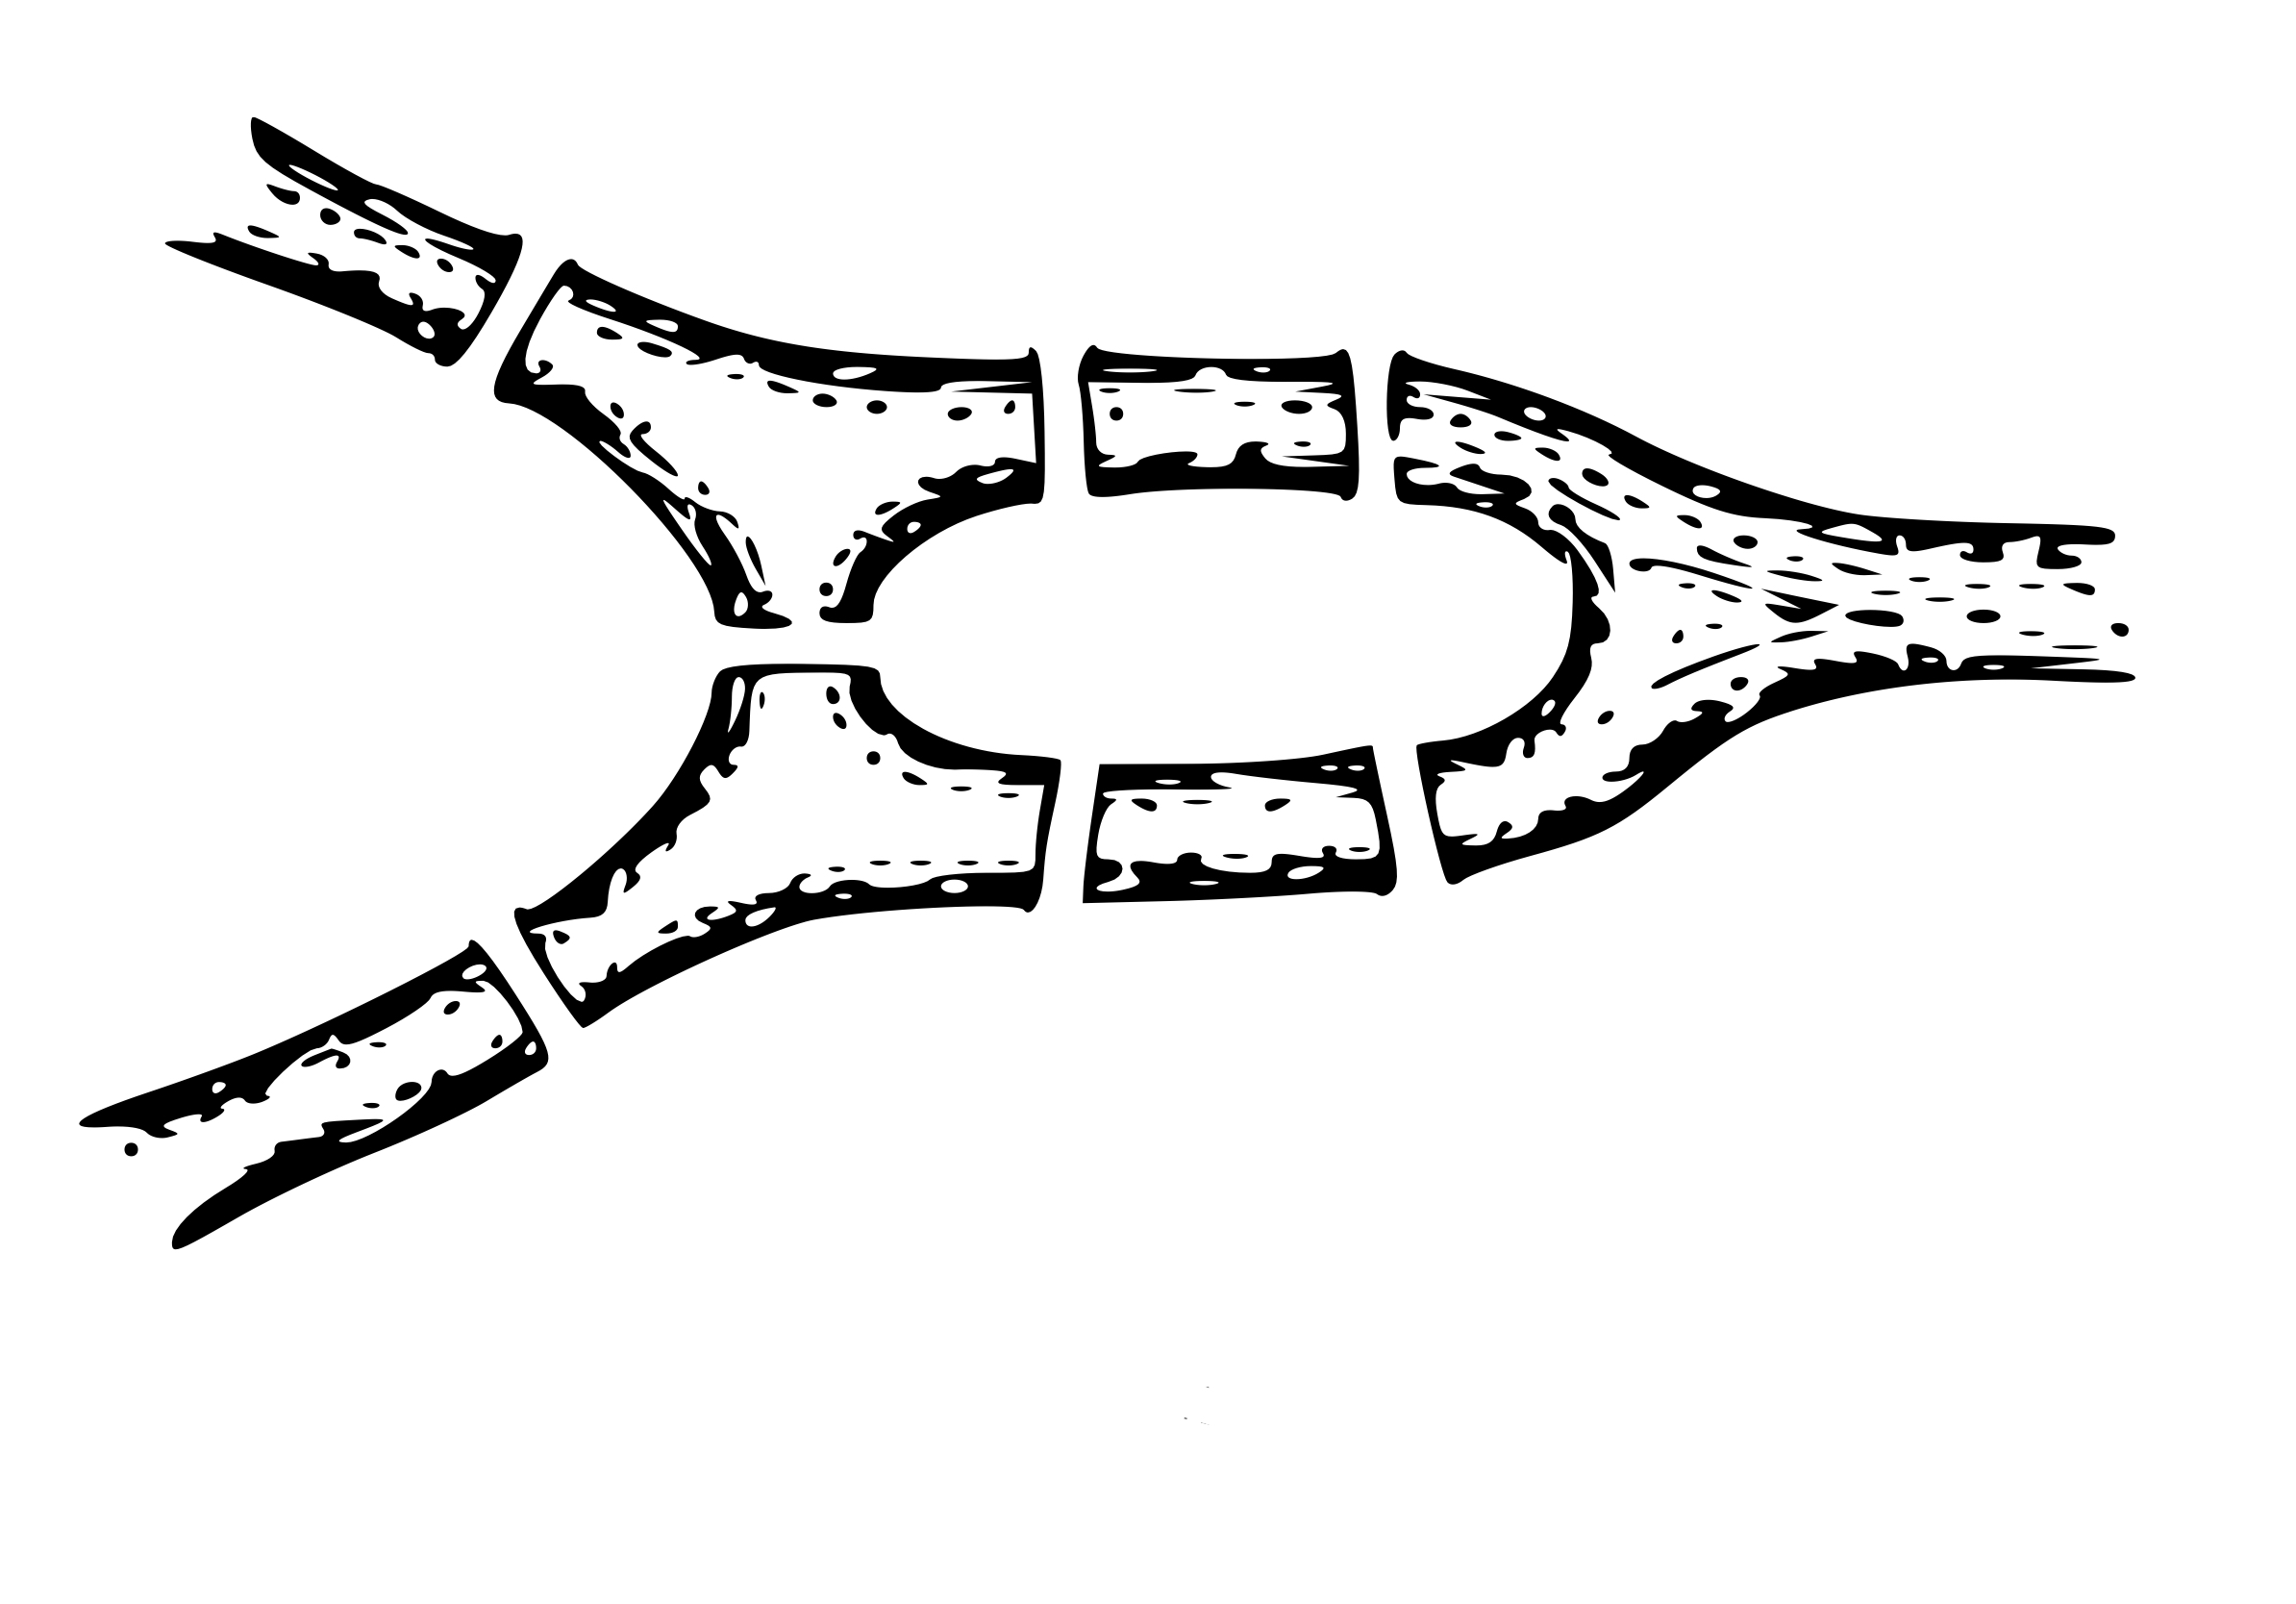
\includegraphics[height=8cm]{Fig4.jpeg}
    \caption[]{}
    \label{Fig4}
\end{figure}

\begin{figure}
    \centering
    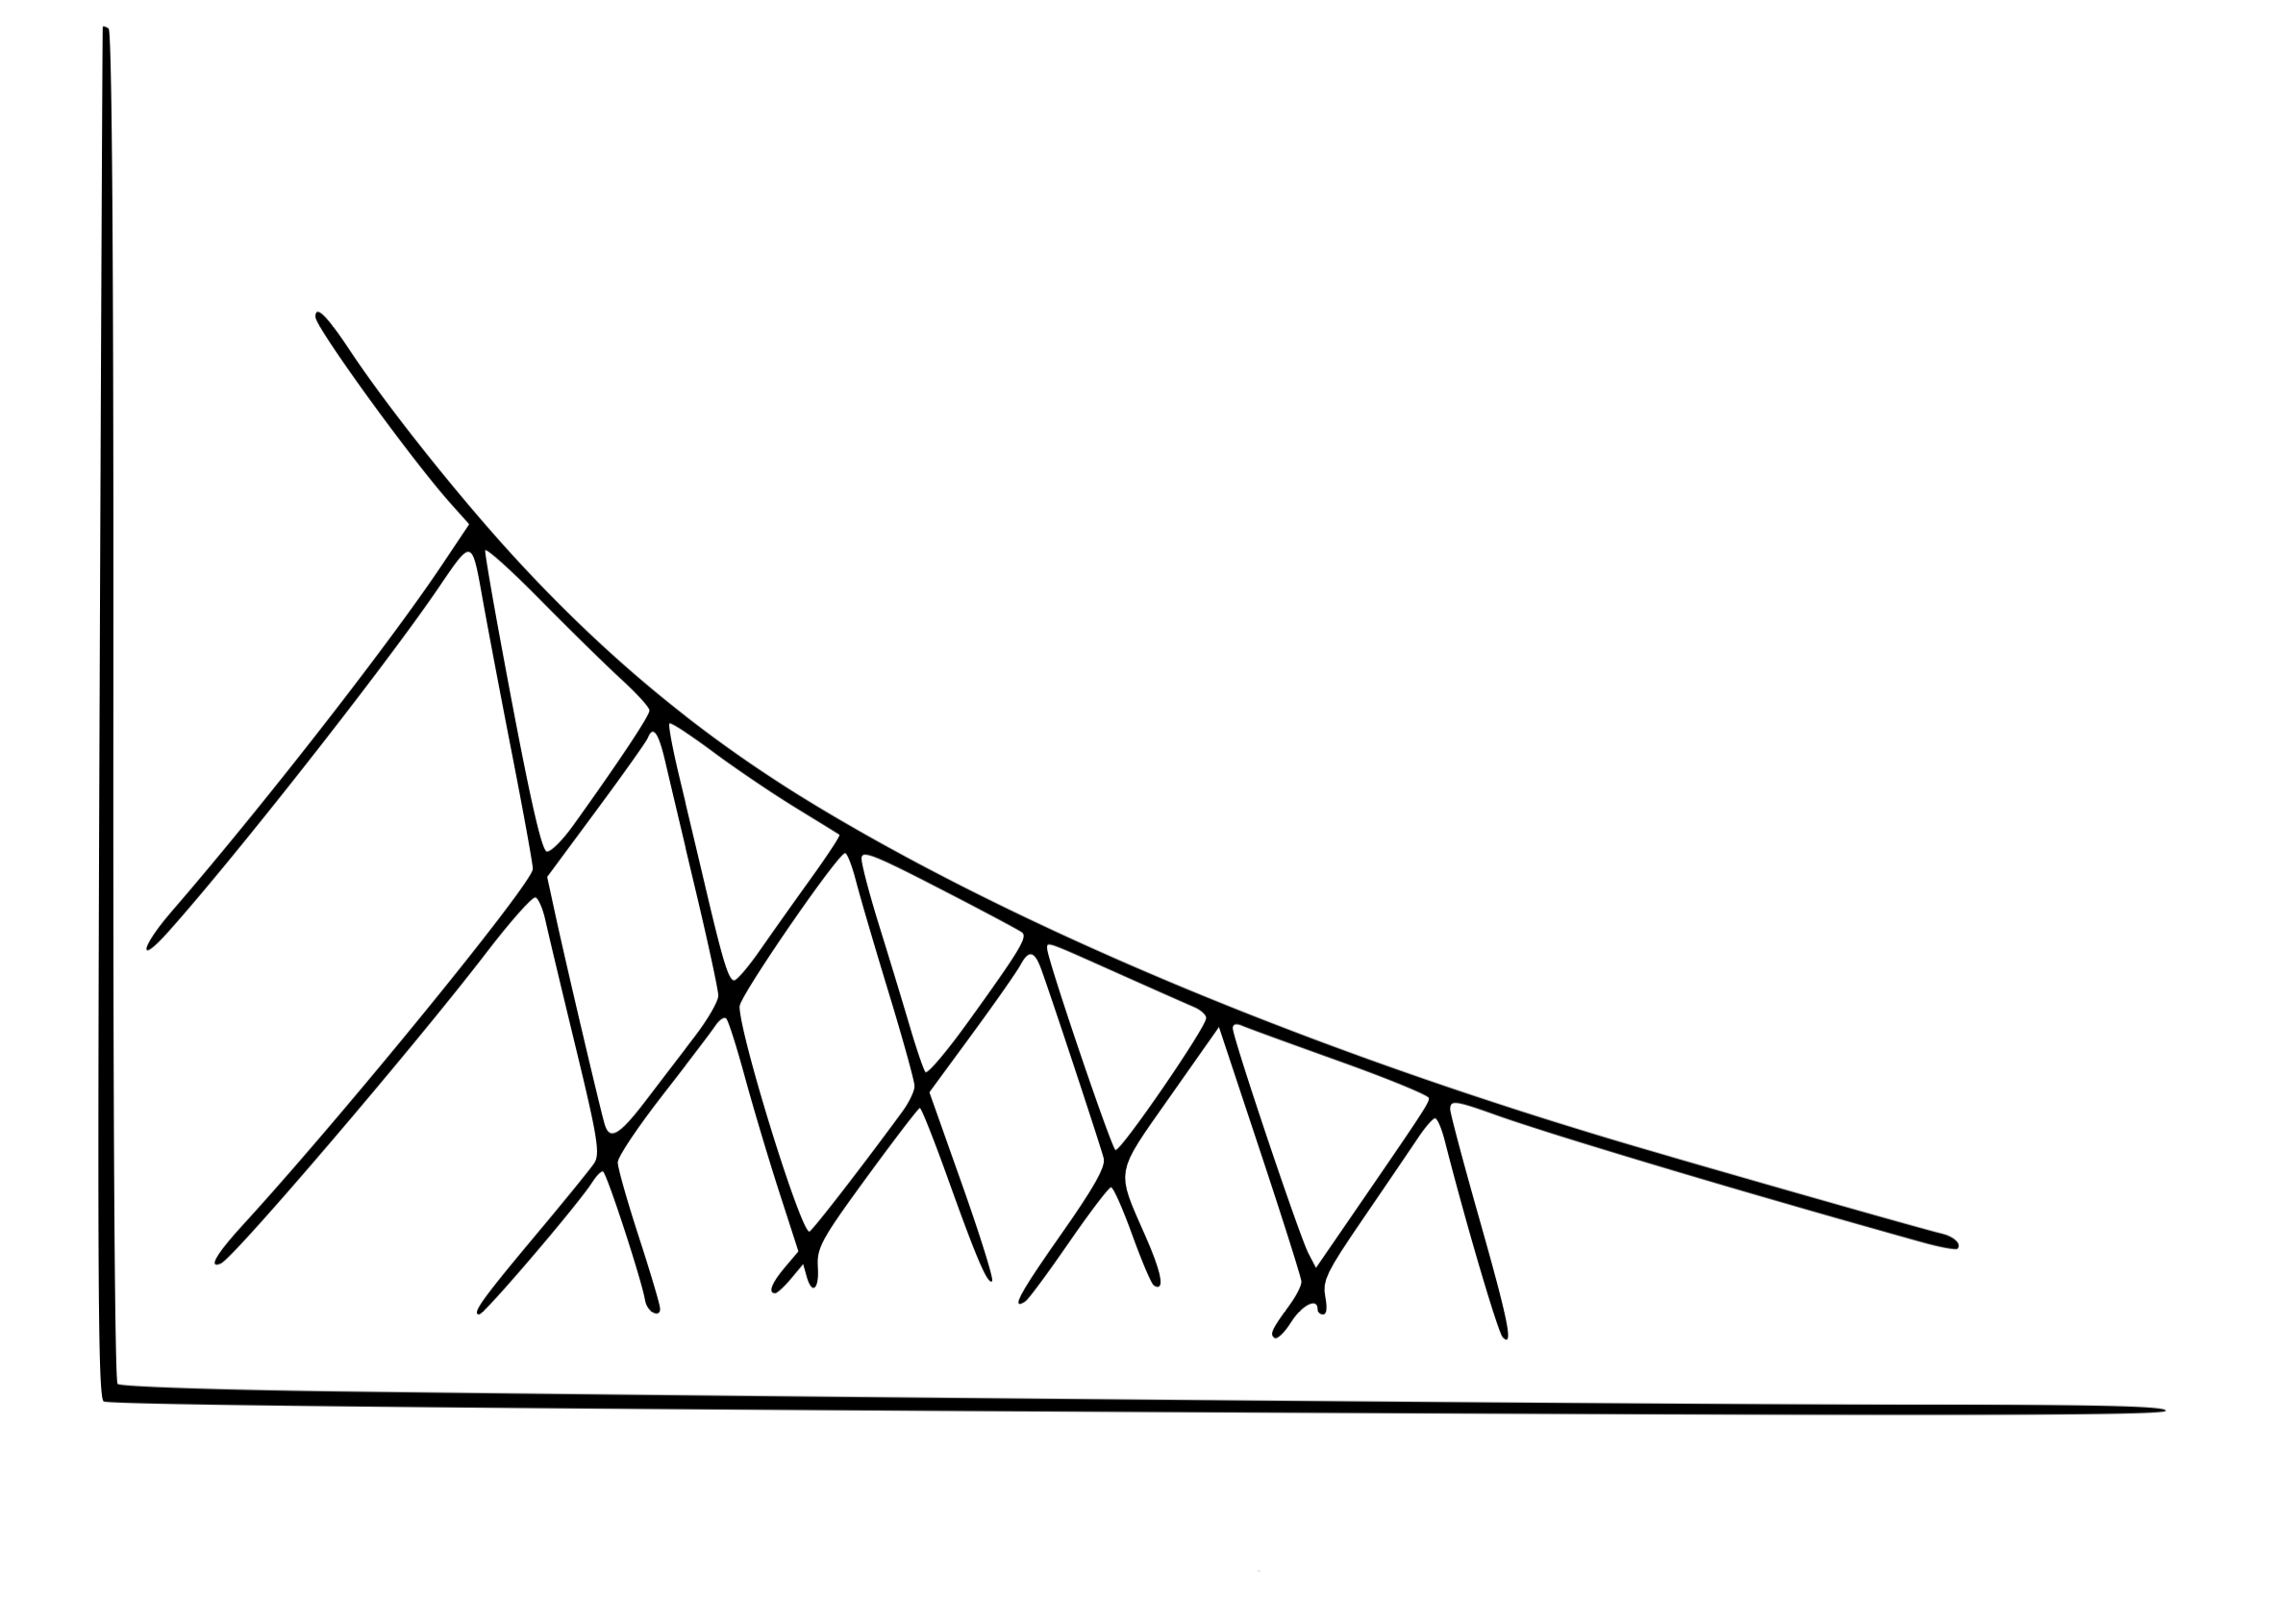
\includegraphics[height=8cm]{Fig5.jpeg}
    \caption{}
    \label{Fig5}
\end{figure}

Equation (\ref{eq1}) defines $y'$ as a function of $x$ and $y$, but this funciton has several determinations or branches. This state of things is not satisfactory from out point of view above. In order to avoid this, let us consider the surface $f(x,y,z)=0$ is space. For each point of that surface, we have
\begin{equation}
    dy/dx=z
    \label{eq3}
\end{equation}
So that the problem becomes to trace on the surface, those curves which have $dy/dx$ equal to $z$. Geometrically speaking, such curves must, in each point, be tangent to a certain direction, viz., the intersection of the tangent plane to the surface with a certain vertical plane (represented by (\ref{eq3})). The system (\ref{eq1}) and (\ref{eq2}) represents the ``horizontal boundary'' of the surface. At each point $m$ on it, the tangent plane is vertical (\ref{Fig6}). What happens there? We see that in $m$, the two planes which define the tangent to our curve are vertical (the plane corresponding to (\ref{eq3}) being to in any case). Therefore, this tangent itself is also vertical. This gives immediately the desired result; for it is well known that by projecting a psace curve on a plane perpendicular to one of its tangents, we obtain a projection curve which has a cusp. The only exception would be when our two planes would coincide and this indeed gives the supplementary condition for the existence of a singular solution. \par

\begin{figure}
    \centering
    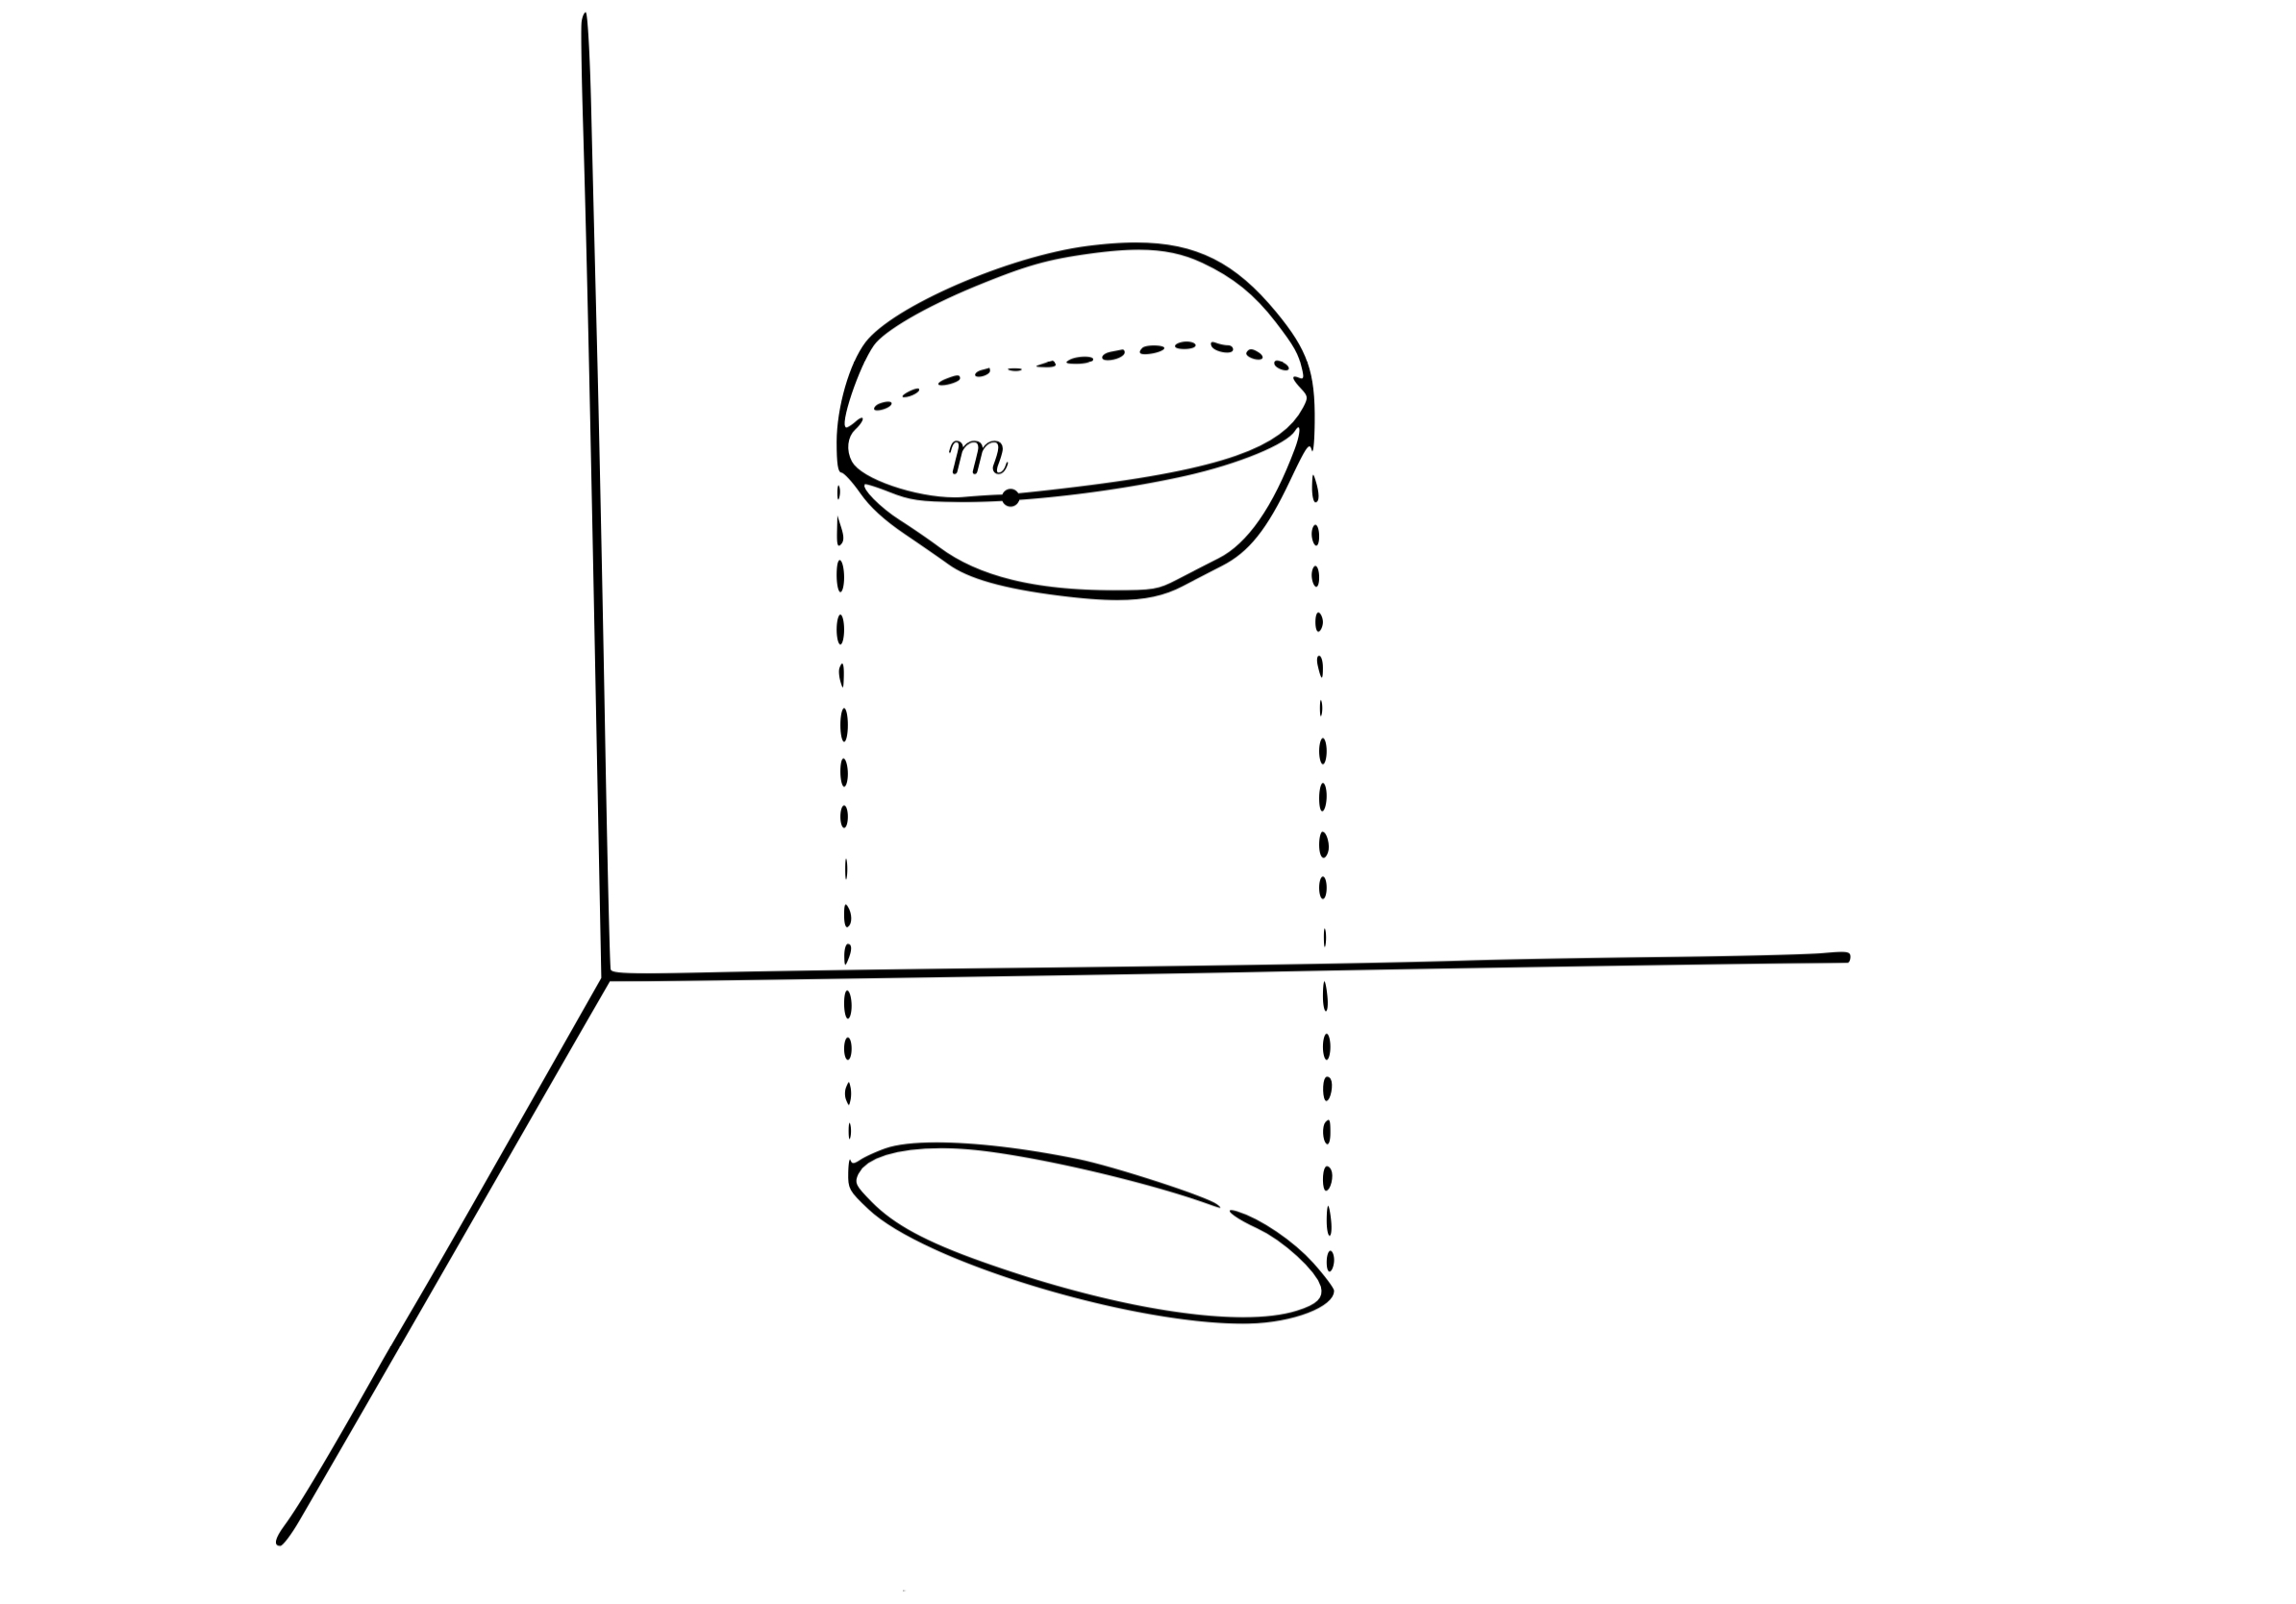
\includegraphics[height=8cm]{Fig6.jpeg}
    \label{Fig6}
\end{figure}

A difficult question in differential equations is thus reconducted to an elementary result of analytical geometry; and this is obtained by the mere fact of depicting correctly (in the sense of Riemann) $y'$ as a function of $x$ and $y$. Only when this adequate representation of the domain of variation is obtained, analysis situs is to be applied. \par

Before seeing it in operation, let us notice tha Cauchy had an opportunity of discovering its importantce. This is a curious historical fact in his worrk; for it was one of his few errors. It was done in his youthful period, when dealing with the theorem of Euler on polyhedrons. This theorem connects the number of faces, summits and edges. It expresses that $F+V=E+2$, where $F$ is the number of edges. Cauchy's demonstration was false, and so is even the theorem itself. This theorem holds efffectively (and this is the reason why Euler and Cauchy believed to be true) for a very large category of polyhedra, among which every convex one occurs. But others had been overlooked, such as those which have the general shape of an anchor ring, and these do not verify the above relation. If Cauchy had perceived that error; if he had noticed tha exception to Euler's theorem, it may be presumed with some probability that he would not have left to Riemann the glory of founding a complete theory of algebraic functions. \par

Let me remind you of the difference between the method of Cauchy (and of Puiseux) and that of Riemann. If we consider the algebraic function defined by $F(x,y)=0$, then $y$, in general, in the environs of $x_0$ and $y_0$, is a regular analytic function of $x$ and is given by a Taylor's series within a ceratin circle around $x_0$. Inside this circle, the principles of Cauchy and Weierstrass permit us to study the function. At critical points $x_1$ , where $y$ is not a holomorphic function of $x$, Puiseux studied this. He took $X=(x-x_1)^\frac{1}{p}$, $p$ being properly chosen. Then $y$ can be developed in powers of $X$ instead of in terms of $x-x_1$. Everything seems at first to be settled then. But really we still ignore some fundamental properties. The reason of this is that we do not get the direct idea of the total domain, but only an indirect idea of it by a series of smaller regions. \par

It is true that these smaller regions are suh that, taken altogether, they cover the totality of the domain in question, and for that reason, they finally may enable us to master it completely. But the error was to believe that this could be without a special study of the manner in which those partial regions are united. \par

I should compare this (though the comparison is very incomplete) to the map of a largy country, which is given by a series of partial leaves. We must take account, not only of each separate leaf, but of the ``assembling table'' showing their general disposition, so as to pass from the detail to the whole. The capital and unexpected fact, the discovery of which belongs to Riemann, is that such ``assembling tables'' are not at all like each other; that there are several quite different kinds of them: therefore, the synthesis of the details of the solution cannot be well understood without noticing thsees differences. \par

\section{}
It is now evident that the importance of these considerations is not limited to algebraic functions. They are connected with every synthesis of the above mentioned kind, that is to say, theoretically speaking, with every employment of integral calculus. \par

They constitute a sort of revenge of geometry on analysis. Since Descartes, we have been accustomed to replace each geometric relation by a corresponding relation between numbers, and this has created a sort of predominance of analysis. Many mathematicians fancy they excapt that predominance and consider themselves as pure geometers in opposition to analysis; but most of them do so in a sense I cannot approve: they simply restrict themselves to treating exclusively by geogetry questions which other geometers would treat, in general quite easily, by analytical means; they are of course, very frequently forced to choose their questions not according to their true scientific interest, but on account of the possibility of such a treatment withot intervention of analysis. I am even obliged to add that some of them have dealt with problems total lacking any interest whatever, this total lack of interest being the sole reason why such problems have been left aside by analysts. Of course, I not only admit geomterical treatment, but use it every time I find it possible, for, if applicable at all, it gives us, in general a much better view of the subject than an analytical one. But very important problems may be inaccessible to it. We must use all means at our disosal and choose, not this or that on \textit{a priori}, but the one besta adapted to our question. \par

But here geometry has over analysis a more certain advantage. I consider that analysis could not, or could only with great difficulty, and probably after a long series of sterile efforts, have replaced the geometrical views we have just alluded to for resolving the corresponding part of the problem. I mean that passage from the solution in small regions to the solution over the whole domain.\footnotemark \par

\footnotetext{Logically speaking, even the results of analysis situs can be rigorously stated in numerical language; but such statements have been made only after the results have been found, and some parts of this analytic treatment are of extreme difficulty (such as Jordan's theorem).}

Let us, for instance, admit that that domain is a two-dimensional one. Then according to analytical methods, we ought to individualize any point of it by giving the values of two parameters, $x$ and $y$. But the representation of a geometrical problem by means of functions of $x$ and $y$ often makes us lose some element of the problem: functions in a domain in two dimensions may be something else than the functions of $x$ and $y$. The simultaneous variation of $x$ and $y$ represents a plane. Now a plane has not the same general shape as a sphere or anchor ring, and those differences are lost in Descartes's method. We can have, for instance, as many examples of this difference in rational dynamics as we please. One knows that when a dynamical problem has two degrees of freedom the corresponding differential equations, i.e. the equations of Legrange, are defined, the parameters which define the position of the system being designated by $x$ and $y$, if one gives the expression $2T=E(x,y)x'^@+2F(x,y)X'y'+G(x,y)y'^2$ for the vis viva and the expression $U=\psi(x,y)$ for the force function. Therefore, if two problems of dynamics correspond to the same expression of $T$ and the same expression of $U$, their studies ought tot be exactly identical and reducible to each other. That matters may  really be quite different is to to be immediately seen by the following example: \par

(1) Consider the material particle acted on by no forces. The trajectories will be straight lines. (2) Let us have a vertical standard. The arms $AA'$ and $BB'$ are solidly attached and $A$ and $B$ are fixed (Fig. 7). The only motion of the system is a rotation about $AB$. $A'B'$ is a second axis about which a rigid body homogeneous and of revolution can rotate. The system has two degrees of freedom. We have to study the motion of the system. There will be no force function. Only rotations are possible (two independent ones around $AB$ and one around $A'B'$). \par

Analytically, the two problems are one and the same, for in both cases, $U=0$ and the coefficients $E,\, F,\, G$ in $2T$ are constants (which can always, by a linear transformation in $x,\, y$, be reduced to $E=G=1,\, F=0$). Nevertheless, there is evidently no comparison between the motions in case (1) and case (2), so that to a certain extent, we are deceived by analytic methods. The assemblage of all possible positions of system (2) can be represented not on a plane, but on the surface of an anchor ring. \par

We know since the researches of Poincar\'e that the study of trajectories represented by differential equations must be founded on analysis situs. For instance, $f(x,y,y')=0$ is geometrically represented by a certain surface, and on this surface defines a geometrical correspondance as follows: for each point of the surface it defines a certain direction (with its sense) in the tangent plane. We have then to draw at each point of the surface a curve which is tangent to the direction thus defined. Poincar\'e showed that such a problem cannot be handled unless we know what the genus of the surface is. This already appears ina simple preliminary question which arises in that study. We have said that we have a certain direction at each point of our surface. Can we \textit{in general} do this without exception? In general, we cannot. In each point, in general, we shall have a certain tangent direction defined, but there will be certain singular points in the correspondence. The only case in which the correspondence can be complete is when the surface is of genus one. For instance, there \textit{must} be singular points for the genus zero. In that case, Poincar\'e stated that every trajectory is either a closed one, or finishes in a singular point, or is asymptotic to a closed curve. For genus one, singular points may be absent, but the shapes of curves verifying the equation may yet be much more complicated. \par

Differential equations of higher order will also of course (and did indeed in some parts of Poincar\'e's work) require the intervention of analysis situs. But the difficulty will be much greater, as in hyper-spaces this theory becomes as complicated as it was simple in Riemann's hands when applied to ordinary surfaces. These higher chapters of analysis situs begin, however, to be well known, and though they could not hitherto be applied to differential equations, their role is already clear, owing to the works of Picard and Poincar\'e, in the natural generalization of Riemann's original theory. I mean the difficult theory of algebraic surfaces and algebraix functions of two or more independent variables. \par

In the line of partial differential equations, we must point out a very remarkable analogous example due to Volterra and concerning the problem of elasticity. Generally speaking, if the external forces and also the peripheric efforts acting on a homogeneous solid body are zero. so will be the stress at every point of its substance. More precisely in such a body of simple connected shape, stress could only appear under those conditions if singular points would exist where they would cease to obey the general laws known for their sitribution. But the contrary can take place if the body has an annular form, and in fact Volterra practically constructed such annular bodies win which stress exists and can be experimentally perceived, without any external action and without any singular point. \par

But examples of a much more elementary character, belonging to the very beginning of the differential calculus, can be give. Let us consider a point-to-point correspoondence, defined by such equations as
$$X=f(x,y),\quad Y=g(x,y).$$
When does that system of equations admit one and only one solution in $x,y$ if $X, Y$ are supposed to be given? \par

It is classical that this, above all depends on the functional determinant
$$\frac{D(X,Y)}{D(x,y)}=
    \begin{vmatrix}
        \frac{\partial f}{\partial x} & \frac{\partial f}{\partial y} \\[0.3em]
        \frac{\partial g}{\partial x} & \frac{\partial g}{\partial y}
    \end{vmatrix}. $$
Suppose that this is not zero in a certain point $x_0,y_0$. We are taught that in a the \textit{neighborhood} of $(X_0,Y_0)$ the system will have one and only one solution. The tempting conclusion is to suppose that if everywhere this determinant is not zero, then everywhere we will have a one-to-one correspondence. This is not true, and indeed errors have been committed on that subject. Even in the simplest casae, in which the representation of the \textit{whole} plane of $XY$ on the \textit{whole} plane of $xy$ is considered, a supplementary condition at infinity must be added in order to ascertain that the transformation is one-to-one. \par

But now let us replace our planes by two spheres, a correspondence being considered between a point $(x,y,z)$ of the surface of the first sphere, and a point $(X,Y,Z)$ of the surface of the second. In this case we find that if a condition analogous to that above holds at every point of the first surface it will actually insure a regular one-to-one correspondence. \par

But if we replace our spheres by two anchor rings, the results will again be completely and utterly changed. Several points on the surface of one anchor ring may correspond to one and the same point on the surface of a second one, although in the neighborhood of each oint everything seems to take place just as in a one-to-one correspondence. To see this, one has only to note that a point on the torus depends on two angles, $\Theta$, $\psi$. If we calle, $\Theta'\psi'$ the two similar angles for the second surface, we have only to define the correspondence by $\Theta'=p\Theta,\, \psi'=q\psi,\, p$ and $q$ being two arbitrary integers.\footnotemark

\footnotetext{It is interesting to add that as far as ordinary (closed) surfaces are concerned, the genus 1 is the only one for which such a paradoxical circumstance can occur, in the sense that, if each point of a closed surface $\Sigma$, of genus $g>1$, corresponds to one (and only one) point of a second closed surface $\Sigma'$ \textit{of the same genus,} and if, in the neighborhood of each point, the relation thus defined takes the character of a one-to-one regular correspondence, it is such on the whole surfaces. \par

This is easily seen in noting that, more generally, if we place ourselves under the same conditions except that we do not suppose the two genera, $g,\, g'$ to be equal, and if $h$ be the number of points of $\Sigma$ corresopnding to the same point on $\Sigma'$, this number $h$ (which must be the same everywhere, on account of the absence of singular points) is connected with $g,\, g'$ by the equation $g-1=h(g'-1)$: a fact which results from the generalizaed Euler's theorem. \par }

A curious fact is that the samet hing occurs with respect to two circles. It is evident that if two points respectively move on the two circumferences with uniform speed, one turning exactly $p$ times ($p$ being an integer) while the other turns once, each position of the former will correspond to $p$ distinct positions of the latter, although the ratio of speeds never changes signs, nor even becomes zero or infinite. \par

Nothing of the kind could, as we saw, occur on the surfaces of our two spheres (nor of two hyperspheres in \textit{n}-dimensional space, if $n>2$), so that, in that respect, the case of two dimensions proves more complicated than that of three or more dimensional spaces. \par

These peculiar distinctions are closely connected with the fundamental distinctions of analysis situs. They are due to the fact that there eare many ways essentially distinct from each other, of passing from one pooint to another of a circumference (according to the number of revolutions performed around the curve) whilst any line joining two points of the surface of a sphere can be changed into any other one by conintuous deformation. \par

This question of coresopndences and Euler's theorem on polyhedra would give us the most simple and elementary instances in which the results are profoundly modified by considerations of analysis situs, if another one did not exist which concerns the principles of geometry themselves. I mean the Klein-Clifford conception of space. But since this conception has been fully and definitively developed in Klein's Evanston Colloquium, there is no use insisting on it. We want only to remember that this question bears to a high degree the general character of those which were spoken of in the present lecture. Klein-Clifford's space and Euclid's ordinary space are not only approximately, but fully and rigorously identical as long as the fugres dealt with do not exceed certain dimensions. Nothing therefore can distinguish them from each other in their infinitesimal properties. Yet they prove quite different if sufficiently great distances are considered. \par

This example, as you see, exactly like the previous ones, teaches us that some fundamental features of mathematical solutions may remain hidden as long as we confine ourselves to the details; so that in order to discover them we must necessarily turn our attention towards the mode of synthesis of those details which introduce the point of view of analysis situs. \par

\chapter[Lecture IV]{Lecture IV\\Elementary Solutions of\\Partial Differential Equations And\\Green's Functions}
\section{Elementary Solutions}

The expressions we are going to speak of are a necessary base of the treatment of every lineasr partial differentia lequation, such as those which arise in physical problems. The simplest of them is the quantity employed in all theories of the classical equation of Laplace: $\nabla^2u-0$; namely the elementary Newtonian potential $1/r$, where
$$r=\sqrt{(x-a)^2+(y-b)^2+(z-c)^2}$$
and $(a,b,c)$ is a fixed point. \par

The potential was really introduced first and gave rise to the study of the equation. All known theories of this equation rest on  this foundation. The analogous equation for the plane is
$$\frac{\partial^2u}{\partial x^2}+\frac{\partial^2 u}{\partial y^2}=0.$$
Here we must consider the \textit{logarithmic potential}, $\log 1/r$, where $r=\sqrt{(x-a)^2+(y-b)^2}$. By this we see that if we wish to treat any other equation of the aforesaid type, we must try to construct again a similar solution which possesses the same properties as $1/r$ possesses in the case of the equation of Laplace. How is such a solution to be found? To understand it, we must examine certain properties of $1/r$. First let us note that that quantity $1/r$ is a function of the coordinates of two points $(x,y,z)$ and $(a,b,c)$ [the corresonding element of $\log 1/r$ in the plane being similarly a function of $(x,y;a,b)$]. If considered as a function of $x,y,z,$ alone ($a,b,c,$ being supposed to be constant) in the real domain, $1/r$ is singular for $r=0$; and $r=0$ only when $x=a,\, y=b,\,\text{and}\, z=c$ simultaneously. But for complex points, $1/r$ is singular when the line that joins $(x,y,z)$ and $(a,b,c)$ is part of the isotropic cone of summit $(a,b,c)$. \par

This isotropic cone is not introduced by chance, and not any surface could be such a surface of singularity. It is what we shall call the \textit{characteristic cone} of the equation. We already met with the notion of characteristics in our first lecture, and saw that it is nothing else than the analytic translation of the physical expression ``waves.'' I must nevertheless come back to it this time in order to remind you that the word ``waves'' has two different senses. The most obvious one is the following: Let a perturbation be produced anywhere, like sound; it is not immediately perceived at every other point. There are then points in space which the action has not reached in any given time, Therefore the wave, in that sense a surface, separates the medium into two portions (regions): the part which is at rest, and the other which is in motion due to the initial vibration. These two portions of space are contiguous. It was only in 1887 that Hugoniot, a French mathematician, who died prematurely, showed what the surface of the wave can be; and even his work was not well known until Duhem pointed out its importance in his work on mathematical physics. \par

A second way of considering the wave is more in use among physicists. We have not in the first definition impled vibrations. If we now suppose that we have to deal with sinusoidal vibrations of the classical form, the motion is general and embraces all the space occupied by the air. Tracing the locus of all points of space in which the phase of the vibration is the same, we determine a certain wave surface (or surfaces). \par

It is clear that these two sense of the word ``waves'' are utterly different. In the first case, we have space divided into two regions where different things take place, which is not so in the second case. Certainly, physically speaking, we feel a certain analogy between them. But for the analyst, there seems to be a gap between the two points of view. \par

The gap is filled by a theorem of Delassus. Let us consider any linear partial differential equation of the second order, and suppose the $u$ is a solution which would be singular along all points of a certain surface, $\pi(x,y,z)=0$. By making some very simple hypotheses as to the nature of the singularity, Delassus found that this surface must be a characteristic as defined in our first lecture; that is, it must verfiy, if the given equation is $\nabla^2u=0$, the (non-linear) partial differential equation of the first order
$$\left(\frac{\partial\pi}{\partial x}\right)^2+\left(\frac{\partial\pi}{\partial y}\right)^2+\left(\frac{\partial\pi}{\partial z}\right)^2=0$$
obtained by substituting for the partial derivatives of the second order of the unknown function $u$ in the given equation, the corresponding squares or products of derivatives of the first order of $\pi$ (the other terms of the given equation being considered as cancelled). This is the \textit{characteristic equation} corresponding to our problem. It is the same as the one found by Hugoniot in studying the problem from the first point of view. This third definition will show us the connection between the first two. In the first case, the wave corresponds to discontinuity, for the speeds and accelerations change suddenly at the wave surface: such a discontinuity is evidently a kind of singularity. In the vibratory motion the general equation contains the factor $\sin\mu\pi$ since $u=F\sin\mu\pi$, where $F$ is the parameter corresponding to the frequency, and $\pi$ is a function of $x,y,z$. This from of $u$ seems to show no singularity, for the sine is a holomorphic function. It is nevertheless what one may call ``practically singular.'' If we suppose that the absolute magnitude of $\mu$ is large, the function varies very rapidly from $+1$ to $-1$, it has derivatives which contain $\mu$ in factor, and these derivatives are therefore very large. It has a resemblance to discontinuous function because of the large slope. So that, in what may be called ``approximative'' analysis, it must be considered as analogous to certain discontinuous functions. From that point of view the three notions of waves are closely connected. \par

This view of Delassus is the one which will interest us now because in the case of the elemetary solution $1/r$ the characteristic cone is a surface of singularity. We see now in what direction we may look for the solution of the problem. We have to find what will be the characteristic cone or surface corresponding to it. Then we must construct a solution habing this as a singularity. The first question is answered by the general theory of partial differential equations of the first order. We must have a conic point at $(a,b,c)$. In general the characteristic cone is replaced by a \textit{characteristic conoid} which has curvilinear generatices which correspond to the physical ``rays.'' Secondly, we must build a solution which will have this for a surface of singularity. The first work of general character in this direction was that of Picard in 1891. He considered the case of two variables and treated more especially the equation
\begin{equation}
    \tag{4.1'}
    \label{eq4.1'}
    \frac{\partial^2 u}{\partial x^2}+\frac{\partial^2u}{\partial y^2}=cu.
\end{equation}
Not every equation of the general type
\begin{equation*}
    A\frac{\partial^2u}{\partial x^2}+B\frac{\partial^2u}{\partial x\partial y}+C\frac{\partial^2u}{\partial y^2}+2D\frac{\partial u}{\partial x}+2E\frac{\partial u}{\partial y}+Fu=0
\end{equation*}
can be reduced to that form. But in the elliptic case ($B^2-AC<0$) it can, by a proper change of independent variables, be reduced to the form
\begin{equation}
    \frac{\partial^2u}{\partial x^2}+\frac{\partial^2u}{\partial y^2}+a\frac{\partial u}{\partial x}+b\frac{\partial u}{\partial y}+cu=0
    \label{eq4.1}
\end{equation}
(in which the characteristic lines are the isotropic lines of the plane). Sommerfeld and Hedrick treated this more general form and showed for \eqref{eq4.1}, as Picard had done for the equation \eqref{eq4.1'}, that there exists an elementary solution, possessing all the essential properties of $\log 1/r$. It is
$$ P\log 1/r+Q,$$
$P$ and $Q$ being regular functions of $x$ and $y$. $P$ has the value 1, $x=a,\, y=b$. In the hypervolic case (real characteristices), the form to which the equation can be reduced is Laplace's form
\begin{equation}
    \frac{\partial^2u}{\partial x\partial y}+\frac{\partial u}{\partial x}+b\frac{\partial u}{\partial y}+cu=0
    \label{eq4.2}
\end{equation}
if the change of variables is real; and the coresponding elementary solution is of the type
$$P\log\sqrt{(x-a)(y-b)}+Q,$$
$P$ and $Q$ having the same significations as above ($P$ is nothing else than the function which plays the chief role in Riemann's method for equation \eqref{eq4.2}). Of course, if imaginary changes were admitted (which is possible only if the coefficients are supposed to be analytic) elliptic equations, as well as hyperbolic ones, could be reduced to the type \eqref{eq4.2} or as well, \eqref{eq4.1}. The only case in which that reduction is not at all possible, is when $B^2-AC=0$, the parabolic case. This is a much more difficult case. It has been treated only recently. There is a new type of elementary solution which was given in 1911 by Hadamard in the \textit{Comptes Rendus}, and for the equation of heat with more than two variables by Georey that same year (in the same periodical). \par

Even if we leave the parabolic case aside, the question has a new difficulty arising becuase it is not possible to simplify by changing variables as before when there are more than two of them, so that we must then treat the general case. The problem was, whowever, first treated in the case of
$$\nabla^2u+a\frac{\partial u}{\partial x}+b\frac{\partial u}{\partial y}+c\frac{\partial u}{\partial z}+1u=0.$$
But not every partial differential equation of the second order in three variables can be reduced to this form. It is important nevertheless. Holmgren obtained a solution in form analogous to $1/r$, namely $P/r$, where $P=1$ for $r=0$. \par



\end{document}
